\chapter{Review of Asymptotic Theory}

This chapter provides some basic definitions and concepts for asymptotic theory. 

%***************************************************
\section{Convergence of Deterministic Sequences}\label{sec:nonstochastic_con}\index{Convergence!deterministic sequences}
%***************************************************

In order to understand the asymptotic behavior of stochastic sequences we need first to refresh some concepts about deterministic (non-random) sequences. Recall that a sequence of nonstochastic real numbers $\left\lbrace a_n\right\rbrace$ converges to $a$ if for any $\epsilon > 0$, there exists $n^* = n^*(\epsilon)$ such that for all $n > n^*$,

\begin{equation*}
	\left| a_n - a\right|<\epsilon, 
\end{equation*}
%
e.g., if $a_n = 2 + 3/n$, then the limit is 2 since $\left| a_n - a\right| =\left| 2 + 3/n - 2\right| = \left|3/n\right|< \epsilon$ for all $n > n^* = 3/\epsilon$. 


\begin{figure}[ht]
  \caption{Convergence of sequence $2 + 3/n$}
    \label{fig:SeqConv}
    \centering
    \begin{minipage}{.9\linewidth}
\begin{knitrout}
\definecolor{shadecolor}{rgb}{0.969, 0.969, 0.969}\color{fgcolor}

{\centering 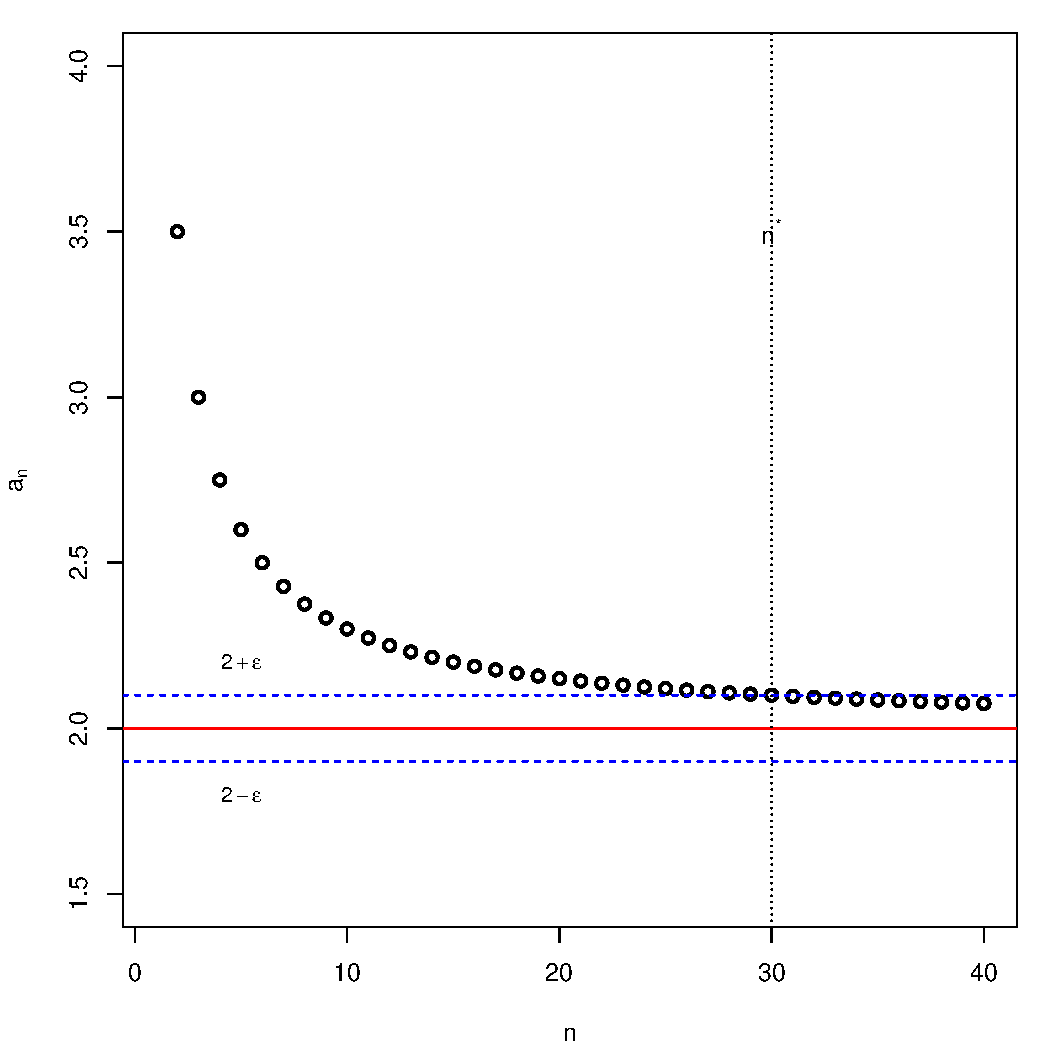
\includegraphics[width=10cm,height=10cm]{figure/SeqConv-1} 

}


\end{knitrout}
\footnotesize
		\emph{Notes: This graphs shows the convergence of the sequence $2 + 3/n$ where $\epsilon = 0.1$ and $a = 2$.}
	\end{minipage}
\end{figure}


Definition \ref{definition:convergence_deterministic} give us a formal statement regarding nonstochastic sequence of numbers.

\begin{definition}[Deterministic convergence]\label{definition:convergence_deterministic}
	The sequence $\left\lbrace b_n: n = 1,2,... \right\rbrace$ of real numbers  converges to the limit $b$ if for every $\epsilon > 0$ there exists and $n^*(\epsilon)$ such that if $n>n^*(\epsilon)$ then $|b_n - b|<\epsilon$. This is also indicated as follows:
\begin{equation*}
\lim_{n\to \infty} b_n = b
\end{equation*}	
\end{definition}

In Definition \ref{definition:convergence_deterministic} by choosing a very small $\epsilon$, we ensure that $b_n$ gets arbitrarily close to its limit $b$ for all $n$ that is sufficiently large. If fact, the smaller $\epsilon$ is, the larger $n(\epsilon)$ will be. So, $\epsilon$ can be interpreted as a prespecified tolerance level for the discrepancy between $b_n$ and $b$. When a limit exists, we say that the sequence $\left\lbrace b_n \right\rbrace$ \textbf{converges} to $b$ as $n$ tends to infinity, written $b_n\to b$ as $n\to \infty$.

Figure~\ref{fig:SeqConv} shows that the sequence $2 + 3/n$ converges to 2. Note that if $\epsilon = 0.1$ then it is always true that $a_n$ will be always between $2 + \epsilon$ and $2 - \epsilon$ if and only if $n \geq n^*= 30$.

In econometric, we talk a lot about sequences of matrices. Probably you are asking yourself, what is a sequence of matrices? Hopefully, the following example will give you some intuition. 

\begin{example}[A sequence of Matrices]\label{example:sequence_matrix}
Let $\mX_n$ be an $n\times 2$ matrix whose $i$th row is defined by the $1\times 2$ vector $\left[1, i\right]$ so that

\begin{equation*}
\mX_n = \begin{pmatrix}
  1 & 1 \\
  1 & 2 \\
  \vdots & \vdots\\
  1 & n
\end{pmatrix}
\end{equation*}

Then

\begin{equation*}
\left\lbrace \begin{pmatrix}
1 & 1\\
1 & 1
\end{pmatrix},
\begin{pmatrix}
  1 & 3/2 \\
  3/2 & 5/2
\end{pmatrix},
\begin{pmatrix}
1 & 2 \\
2 & 14/3
\end{pmatrix}, ...
\right\rbrace
\end{equation*}
%
is a sequence of matrices $\mY_1, \mY_2, \mY_3,...$ defined by the function $\mY_n = \frac{1}{n}\mX_n^\top\mX_n$, where the $n$th element of the sequence is defined as

\begin{equation*}
\mY_n = \begin{pmatrix}
1 & \frac{\sum_{i = 1}^n i}{n} \\
\frac{\sum_{i = 1}^n i}{n} & \frac{\sum_{i = 1}^n i^2}{n}
\end{pmatrix} = 
\begin{pmatrix}
1 & \frac{(n + 1)}{2} \\
\frac{(n + 1)}{2}& \frac{(n +1)(2n +1)}{6}
\end{pmatrix}
\end{equation*}
\end{example}

Now, we formally state the concept of convergence for matrices. 

\begin{definition}[Limit of a Real-Valued Matrix Sequence]
Let $\left\lbrace\mX_n \right\rbrace$ be a sequence whose elements are $q\times k$ real-valued matrices. Suppose there exists a $q\times k$ matrix of real numbers $\mX$ such that $\mX_n\left[i, j\right]\to \mX\left[i, j\right]$ for $i = 1,...,q$ and $j = 1,...,k$. Then the matrix $\mX$ is the limit of the matrix sequence $\left\lbrace\mX_n \right\rbrace$ as $n\to \infty$. If the limit does not exists, the sequence is said to be divergent
\end{definition}

The definition of the limit implies that for a sufficiently large choice of $n$, the matrix $\mX_n$ becomes arbitrarily close to the matrix $\mX$, \textbf{element by element}.


Sometimes, some sequences does not have a limit, but we can say whether they are \textbf{bounded}: 

\begin{definition}[Bounded sequence]\label{definition:bounded_sequence}\index{Convergence!bounded sequences}
 A  sequence $\left\lbrace b_n: n = 1,2,... \right\rbrace$ is \emph{bounded} if and only if there is some $a < \infty$ such that $\left|b_n\right|\leq a$ for all $n = 1,2,...$ Otherwise, we say that $\left\lbrace b_n \right\rbrace$ is \emph{unbounded}.
\end{definition}

Thus, for a sequence of real numbers to be bounded, there must exist a positive number that is larger than the absolute value of each and every number in the sequence. For a sequence that has no limit and is also unbounded, we write $b_n \to \infty$, denoting that the sequence diverges to infinity. 


\begin{example}[Bounded Sequences]
Consider $a_n = (-1)^n$, then $a_n$ does not have a limit, but it is bounded since $-1 \leq a_n \leq 1$. The sequence $a_n = 1/n$ is bounded, since $0 \leq a_n\leq 1$ for all $n = 1,2,...$
\end{example}


\begin{example}[Boundedness and Limit of Matrices]
Consider the following examples:
\begin{enumerate}
 \item Recall the sequence of matrices in Example \ref{example:sequence_matrix}. In this case, only the sequence $\left\lbrace \mY_n\left[1, 1\right]\right\rbrace$ is bounded. All other sequences of matrix elements are unbounded and, in fact, diverge to infinity. Since all the sequences of matrix elements must be bounded for the matrix sequence to converge, the matrix does not have a limit.
 \item Let $\left\lbrace \mX_n\right\rbrace$ be a sequence of matrices such that
 
\begin{equation*}
\mX_n = \begin{pmatrix}
  3n^{-1} & n^{-1} \\
  3       & 1 + n^{-1}
\end{pmatrix}.
\end{equation*}

All four sequences of the matrix elements are bounded, since $\left|3n^{-1}\right|\leq 3$, $\left|n^{-1}\right|\leq 1$, $\left|3\right|\leq 3$, and $\left|1 + n^{-1}\right|\leq 2$, for all $n$. Furthermore, limits exists for all four sequences of matrix elements, since $3n^{-1}\to 0, n^{-1}\to 0, 3\to 3$, and $1 + n^{-1}\to 1$. Thus 

\begin{equation*}
\mX_n\to \mX= \begin{pmatrix}
0 & 0 \\
3 & 1
\end{pmatrix}
\end{equation*}
 \end{enumerate}
\end{example}

Often it is useful to have a measure of the \emph{order of magnitude} of a particular sequence without particularly worrying about its convergence. 
\begin{definition}[Big and little O]\label{definition:big_little_oh}\index{big O}
Consider the following definitions:
	\begin{enumerate}
		\item A sequence $\left\lbrace x_n \right\rbrace $ is $O(n^{\lambda})$ (at most of order $n^{\lambda}$) if $n^{-\lambda}x_n$ is bounded. When $\lambda=0$, $\left\lbrace x_n \right\rbrace $ is bounded, an we also write $x_n=O(1)$.
		\item $\left\lbrace x_n \right\rbrace $ is $o(n^{\lambda})$ if $n^{-\lambda}x_n\to 0$. When $\lambda=0$, $x_n$ converges to zero, and we also write $a_n=o(1)$.
		\item If $\left\lbrace X_n\left[i,j\right]\right\rbrace$ is $O(n^\lambda)$ or $o(n^\lambda)$ for all $i$ and $j$, then the matrix sequence $\left\lbrace \mX_n\right\rbrace$ is said to be $O(n^\lambda)$ or $o(n^\lambda)$
	\end{enumerate}
\end{definition}

The big $O$ notation describes the asymptotic behavior of functions. Basically, it tells you how fast a function grows or declines. 

\begin{remark}
From the definitions we can say that if $X_n = o(n^\lambda)$, then $X_n = O(n^\lambda)$. In other words, \textbf{any convergent sequence is bounded}. The opposite is not true. Recall the example $a_n = (-1)^n$.
\end{remark}

\begin{example}[Order of Magnitude of a Sequence]
Consider the following examples:

\begin{enumerate}
  \item Let $\left\lbrace x_n\right\rbrace$ be defined by $x_n = 3n^3 - n^2 + 2$. Then $\left\lbrace x_n\right\rbrace$ is $O(n^3)$, since $n^{-3}x_n = 3 - n^{-1} + 2n^{-3}$ is bounded. Also $\left\lbrace x_n\right\rbrace$ is $o(n^{3 + \epsilon})$ for any $\epsilon > 0$ since $n^{ - 3 - \epsilon}x_n = 3n^{-\epsilon} - n^{-1 - \epsilon} + 2n^{-3 - \epsilon}\to 0$. For example, Figure \ref{fig:SeqConvBond} plots $n^{-3}x_n$, which is bounded between 4 ($n = 1$) and 2.75 $(n = 2)$. Note also that if we choose $\epsilon = 0.1$, then $n^{3.1}x_n$ clearly converges to 0.
  \item Let $\left\lbrace x_n\right\rbrace$ by defined by $x_n = 3 + n^{-1}$. Then $\left\lbrace x_n\right\rbrace$ is $O(1)$, since $x_n$ is bounded, and $\left\lbrace x_n\right\rbrace$ is $o(n^\epsilon);\forall \epsilon > 0$, since $n^{-3}x_n = 3n^{-\epsilon} + n^{-1 - \epsilon}\to 0$. 
  \item Let the vector sequence $\left\lbrace \vx_n\right\rbrace$ by defined by
  
  \begin{equation*}
    \begin{pmatrix}
    \vx_n\left[1\right] \\
    \vx_n\left[2\right]
    \end{pmatrix}= 
    \begin{pmatrix}
      3n^{-1} \\
      n^{-1}
    \end{pmatrix}.
  \end{equation*}
  Then the vector sequence $\left\lbrace \vx_n\right\rbrace$ is $o(1)$ and $O(1)$, since
  
  \begin{equation*}
    \vx_n \to \begin{pmatrix} 0 \\ 0 \end{pmatrix}
  \end{equation*}
\end{enumerate}
\end{example}

\begin{figure}[ht]
  \caption{Bounded sequence}
    \label{fig:SeqConvBond}
    \centering
    \begin{minipage}{.9\linewidth}
\begin{knitrout}
\definecolor{shadecolor}{rgb}{0.969, 0.969, 0.969}\color{fgcolor}

{\centering 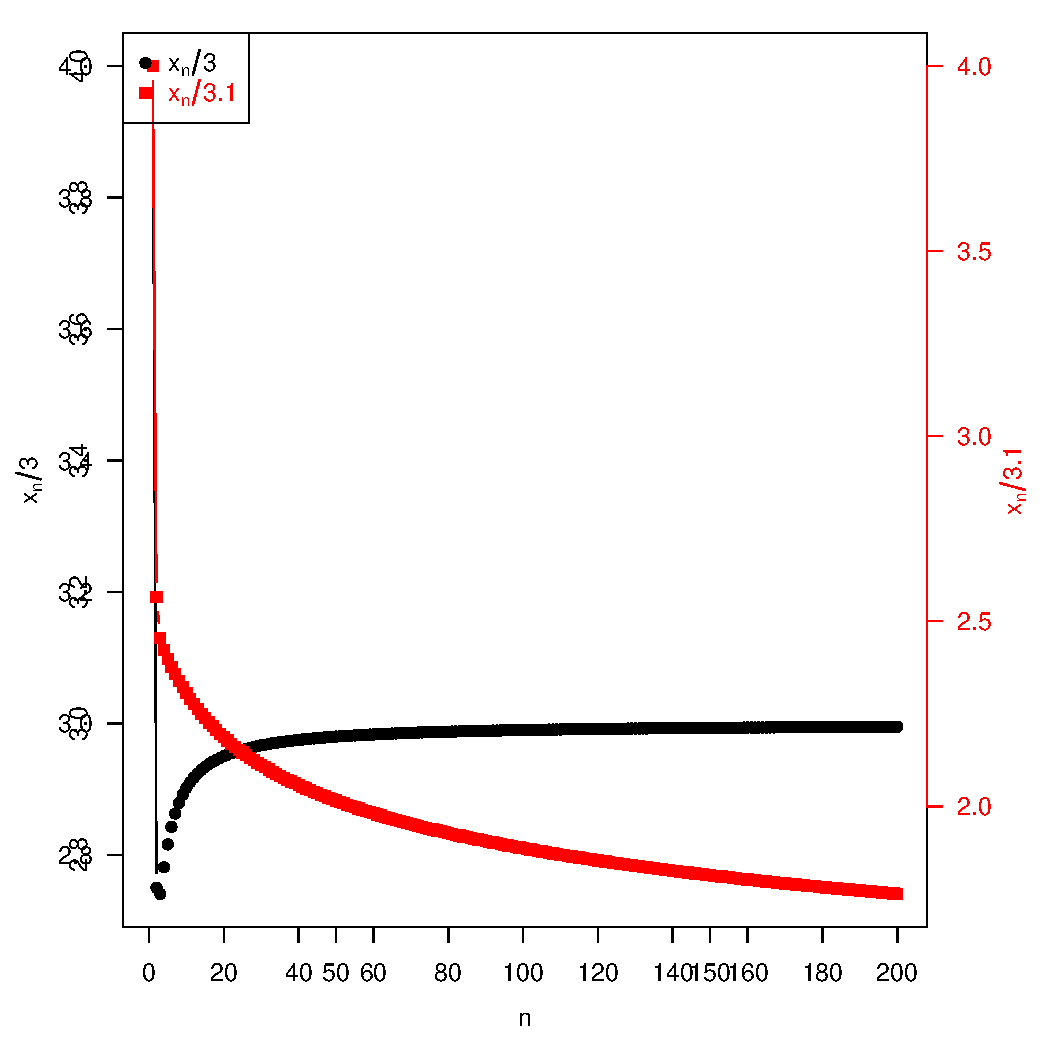
\includegraphics[width=10cm,height=10cm]{figure/SeqConvBoun-1} 

}


\end{knitrout}
\footnotesize
		\emph{Notes: This graphs shows that the sequence $\left\lbrace x_n\right\rbrace$ defined by $x_n = 3n^3 - n^2 + 2$ is $O(n^3)$ and $o(n^{3 + \epsilon})$. For plotting $\epsilon = 0.1$ was selected.}
	\end{minipage}
\end{figure}


%*****************************************
\section{Convergence in Probability}
%****************************************** 

In the previous section we reviewed how a sequence of real number converges to a real number.  What about the sequence of random variables such as econometric estimators? When considering a sequence of \emph{random variables} we cannot be certain that $\left| a_n - a\right|<\epsilon$, even for large $n$, due to the \textbf{randomness}. Instead, we require that \textbf{the probability of being within $\epsilon$ is arbitrarily close to one} as $n\to \infty$. The next definition is more appropriate for convergence in random variables. 

\begin{definition}[Convergence in Probability]\label{definition:convergence_in_probability}\index{convergence in probability}
	A sequence of random variables $\left\{X_n\right\}$ \textbf{convergence in probability} to a constant (non-random) $\alpha$ if, for any $\epsilon>0$,
	
	\begin{equation*}
	\lim_{n\to \infty} \Pr(\left|X_n-\alpha\right|>\epsilon)=0
	\end{equation*}
	
	The constant $\alpha$ is called the \textbf{probability limit} of $X_n$ and is written as $\plim X_n=\alpha$ or $X_n\pto \alpha$. Evidently,
	
	\begin{equation*}
	X_n\pto \alpha\qquad\mbox{is the same as}\qquad X_n-\alpha\pto 0
	\end{equation*}	
\end{definition}

Thus, roughly, convergence in probability states that for large $n$, the probability is high that $X_n$ will be close $\alpha$.

This definition can be understood if we look at Figure \ref{fig:convinprob}. Note that the expression $\left|X_n-\alpha\right|>\epsilon$ can be true or false. The probability that it is true is given by the distribution $F_n(\cdot)$ of $X_n$. Figure \ref{fig:convinprob} shows that the probability that $\left|X_n-\alpha\right|>\epsilon$,  denoted by the red-dashed area outside the interval $\alpha \pm \epsilon$, becomes smaller as $n$ increases. Conversely, the probability of $\left|X_n-\alpha\right|<\epsilon$, given by the blue-dashed area, will become higher and higher as $n\to \infty$. In the limit, this probability should be equal to 1. That is:

\begin{equation*}
	\lim_{n\to \infty} \Pr(\left|X_n-\alpha\right|<\epsilon)=1
\end{equation*}

\begin{figure}[ht]
  \caption{Illustration of convergnce in probability to a constant}
    \label{fig:convinprob}
    \centering
    \begin{minipage}{.9\linewidth}
\begin{knitrout}
\definecolor{shadecolor}{rgb}{0.969, 0.969, 0.969}\color{fgcolor}

{\centering 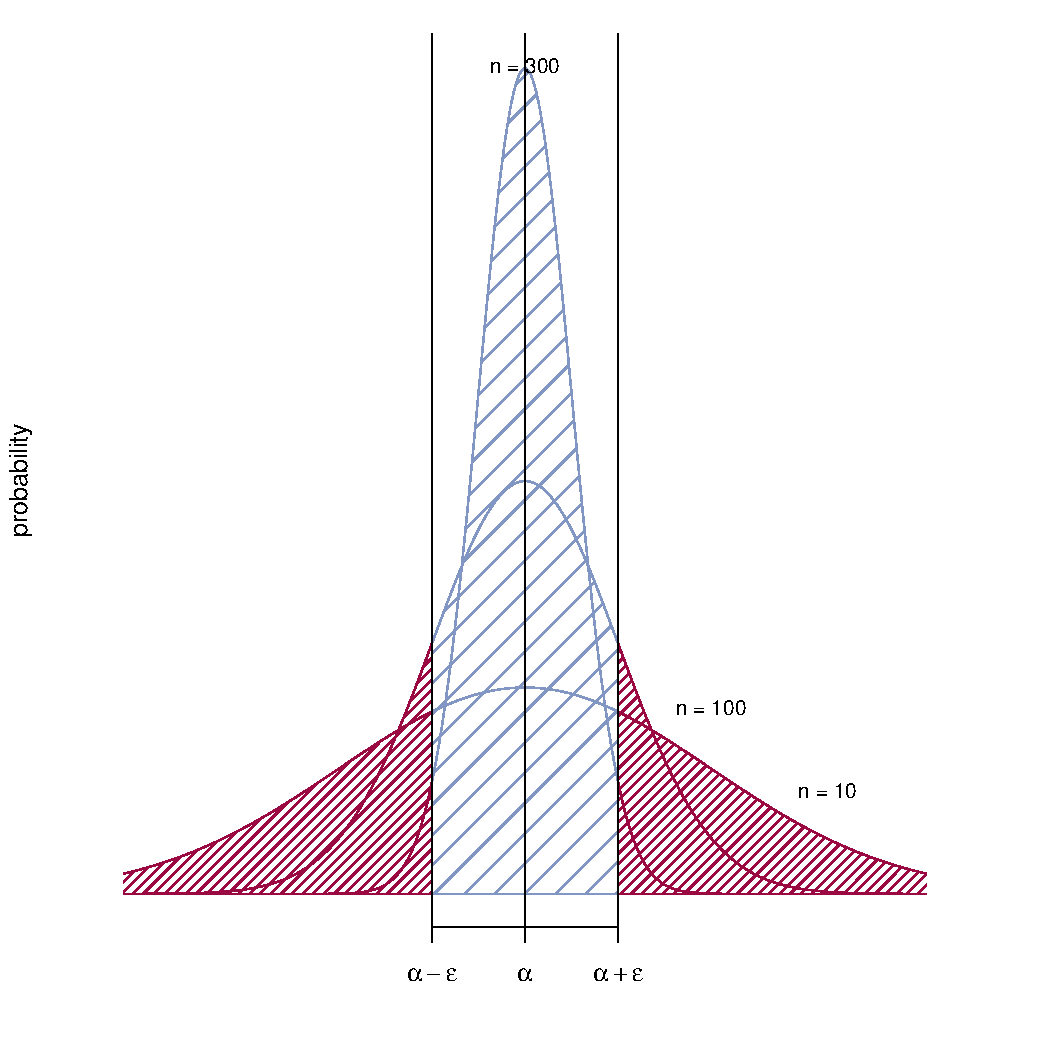
\includegraphics[width=10cm,height=10cm]{figure/convinprob-1} 

}


\end{knitrout}
\footnotesize
		\emph{Notes: This graphs shows that the probability of $\left|X_n-\alpha\right|>\epsilon$, which is denoted by the red-dashed areas, becomes smaller as $n$ increases. }
	\end{minipage}
\end{figure}

Definition (\ref{definition:convergence_in_probability}) can be easily extended to a sequence of random vectors or random matrices (by viewing a matrix as a vector whose elements have been rearranged) by requiring element-by-element convergence in probability. That is, a sequence of $k$-dimensional random vectors $\left\{\vx_n\right\}$ convergences in probability to a $k$-dimensional vector of constants $\valpha$ if, for any $\epsilon>0$,

\begin{equation*}
\lim_{n\to \infty} \Pr(\left\lVert\vx_{n}-\valpha\right\rVert>\epsilon)
\end{equation*}

Note that $\left\| \vx_n - \valpha\right\| $ is the Euclidean distance 

\begin{equation*}
\left[\left(\vx_n - \valpha\right)'\left(\vx_n - \valpha\right)\right]^{1/2} = \sqrt{(x_{1n}-\alpha_1)^2 + ... + (x_{Kn} - \alpha_K)^2} = \left\| \vx_n - \valpha\right\| 
\end{equation*}


Therefore, 

\begin{equation*}
\vx_n \pto \valpha\quad \mbox{iff}\quad \Pr\left[\sqrt{\sum_{j = 1}^k\left(x_{j,n}- x_j\right)^2}> \epsilon\right]\pto 0
\end{equation*}
%
as $n\to \infty$ for $\epsilon >0$ and $\forall j = 1,...,k$, where:

\begin{equation*}
\vx_n = \begin{pmatrix}
          x_{1n} \\
          \vdots \\
          x_{kn}
        \end{pmatrix}
        \quad
        \mbox{and}
        \quad
\valpha = \begin{pmatrix}
            \alpha_1 \\
            \vdots \\
            \alpha_{k}
          \end{pmatrix}
\end{equation*}

\begin{remark}
  $\vx_n \pto \valpha$ if and only if $x_{jn}\pto \alpha_j$ for $j =1, ...,k$. That is, vector convergence in probability is equivalent to component convergence in probability for each component. See our previous discussion of vector sequence.
\end{remark}

\begin{definition}[Probability Limits of Matrices (and Vectors for $k = 1$)]
Let $\left\lbrace \mY_n \right\rbrace$ be a sequence of $m\times k$ random matrices. Then

\begin{equation*}
  \plim \begin{pmatrix}
          Y_n\left[1, 1\right] & \hdots & Y_n\left[1, k\right] \\
          \vdots & \ddots & \vdots \\
          Y_n\left[m, 1\right] & \hdots & Y_n\left[m, k\right]
        \end{pmatrix} = \begin{pmatrix}
          \plim Y_n\left[1, 1\right] & \hdots & \plim Y_n\left[1, k\right] \\
          \vdots & \ddots & \vdots \\
          \plim Y_n\left[m, 1\right] & \hdots & \plim Y_n\left[m, k\right]
        \end{pmatrix}
\end{equation*}
\end{definition}

The expectation $\E(\cdot)$ is a linear operator, that is, \textbf{we cannot} state that $\E\left[\exp(\widehat{\theta})\right] = \exp\left[\E\left(\widehat{\theta}\right)\right]$. Thus, we would like to know if the $\plim$ has the same property. Fortunately, the continuous mapping theorem tell us that we can interchange them. 

\begin{theorem}[Continuous Mapping Theorem]\label{teo:continuous_prob}
	Given a continuous function $g(X)$, if $X_n\pto X$ then $g(X_n)\pto g(X)$ as $n\to \infty$, or equivalently, $\plim \left[g(X_n)\right] = g\left[\plim (X_n)\right]$.
\end{theorem}

The Continuous Mapping Theorem is a very useful theorem. Unlike the expectation operator, it shows that the $\plim$ operator passes through nonlinear functions, provided they are continuous. The lack of this property for the $\E$ operator makes finite sample analysis difficult for many estimators. 


It is useful to know the vector form of this Theorem. Let $\vg:\SR^K\to\SR^J$ be a function continuous at some point $\valpha \in \SR^K$. Then, 

\begin{equation*}
  \vx_n \pto \valpha \implies \vg(\vx_n)\pto \vg(\valpha),
\end{equation*}
%
if $\vg(\cdot)$ is continuous at $\plim \vx_n$.


Now that we have presented the meaning of convergence in probability, it is time to define what we understand for ``consistency'' in econometrics.

\begin{definition}[Consistent Estimator]\label{def:consistent_est}\index{consistent estimator}
  An estimator $\widehat{\vtheta}_n$ of a parameter $\vtheta$ is a consistent estimator $\vtheta$ if and only if
  
  \begin{equation*}
    \plim \widehat{\vtheta}_n = \vtheta,
  \end{equation*}
%
which can also be written as:

  \begin{equation*}
    \widehat{\vtheta}_n \pto \vtheta.
  \end{equation*}
  
\end{definition}

In words, a \textbf{consistent estimator} is an estimator---a rule for computing estimates of a parameter $\vtheta$---having the property that as the number of data used increases without bound, the resulting sequence of estimates converges in probability to $\vtheta$. This means that the distributions of the estimates become more and more concentrated near the true value of the parameters being estimated, so that the probability of the estimator being arbitrary close to $\vtheta$ converges to one. 

\begin{remark}
Convergence in probability is also referred to as weak consistency, and since this has been the most familiar stochastic convergence concept in econometric, the word ``weak'' if often simply dropped.
\end{remark}



\begin{definition}[Strong Convergence in Probability]
	A sequence of random variables $\left\{X_n\right\}$ \textbf{convergence in probability strongly, or, almost surely} to a constant (non-random) $\alpha$ if, for any $\epsilon>0$,
	
	\begin{equation*}
	 \Pr\left(\lim_{n\to \infty}X_n = \alpha\right)=1
	\end{equation*}
	
	This is written $X_n\asto \alpha$, as $n\to \infty$. An equivalent condition for almost sure convergence is
	
	\begin{equation*}
	  \lim_{n\to \infty}\Pr\left(\left|X_m \to X\right| < \epsilon, \forall m\geq n\right) = 1
	\end{equation*}
\end{definition}

The extension to random vector is analogous to that for convergence in probability. Note also that this concept is stronger than convergence in probability; that is, if a sequence converges almost surely, the it converges in probability. 

\begin{remark}
  $\asto \implies \pto$
\end{remark}


In the previous definitions of convergence, the limit is a constant (i.e., a real number). The limit can be a random variable. We say that a sequence of $K$-dimensional random variables $\left \lbrace \vx_n\right\rbrace$ converges to a $k$-dimensional random variable $\vx$ and write $\vx_n\pto \vx$ if $\left\lbrace \vx_n - \vx\right\rbrace$ converges to $\vzeros$. The same applies for almost sure convergence.


We will make frequent use of a special case of convergence in probability, \textbf{convergence in mean square} or \textbf{convergence in quadratic mean}

\begin{theorem}[Convergence in Quadratic Mean]\label{teo:conv_qm}
If $X_n$ has mean $\mu_n$ and variance $\sigma^2_n$ such that the ordinary limits of $\mu_n$ and $\sigma^2_n$ are $c$ and 0, respectively, then $X_n$ converges in mean square to c,

\begin{equation*}
  X_n\qmto c
\end{equation*}
%
and 

\begin{equation*}
  \plim X_n = c.
\end{equation*}
\end{theorem}

This theorem implies that $X_n\qmto c \implies X_n\pto c$. The conditions for convergence in mean square are usually easier to verify than those for the more general form.

The vector form of this type of convergence is the following. We say that the sequence of random vectors $\vx_1, \vx_2,...,\vx_n$ converges in quadratic mean to the random vector $\vz$ if $\E(\vx_n\vx_n')$ and $\E(\vx\vx')$ exists for all $n$ if

\begin{equation*}
  \lim_{n\to \infty} \E\left[\left(\vx_n  - \vx\right)'\left(\vx_n  - \vx\right)\right] = \vzeros
\end{equation*}

A special case of convergence in quadratic mean occurs when $\vx$, instead of being a random vector, is a vector of unknown parameters, say $\vtheta$, and $\vx_n$ is an estimator for $\vtheta$. Under these circumstances we can write:

\begin{equation}\label{eq:biase_var}
  \begin{aligned}
    \E\left[\left(\vx_n  - \vx\right)'\left(\vx_n  - \vx\right)\right] & = \left(\E\left[\vx_n\right]  - \vtheta\right)'\left(\E\left[\vx_n\right]  - \vtheta\right) + \E\left[\left(\vx_n - \E\left[\vx_n\right]\right)'\left(\vx_n - \E\left[\vx_n\right]\right)\right] \\
    & = \sum_{k = 1}^K\mbox{bias}^2(x_{kn}) + \sum_{k = 1}^K \var(x_{kn})
  \end{aligned}
\end{equation}
%
where $x_{kn}$ is the $k$th element of $\vx_n$ that is assumed to be $K$ dimensional. Thus from (\ref{eq:biase_var}) $\vx_n$ converges to $\vzeros$ in quadratic mean if and only if the bias and variance of $\vx_n$ approach zero as $n\to\infty$. This result, and the fact that Chebyshev's inequality can be used to prove that convergence in quadratic mean implies convergence in probability. See below.

Another definitions that will be useful to show other ways of convergences are the Chebyshev's inequality and Markov's inequality.

\begin{definition}[Chebyshev's inequality]\label{definition:chebyshev_ineq}
	 If $X_n$ is a random variable with mean $\mu$ and \textbf{finite variance}, then, for every $\delta > 0$,
	 
	 \begin{equation*}
	 \Pr\left[\left| X_n - \mu\right|\geq \delta \right]\leq \frac{\E\left[(X_n - \mu)^2\right]}{\delta ^2}
	 \end{equation*}
\end{definition}

To prove the Chebyshev inequality, we use the Markov's Inequality

\begin{definition}[Markov's inequality]\label{definition:chebyshev_ineq}
	 If $X_n$ is a nonnegative random variable, then for every $\delta > 0$,
	 
	 \begin{equation*}
	 \Pr\left[X_n \geq \delta \right]\leq \frac{\E\left[X_n\right]}{\delta}
	 \end{equation*}
\end{definition}


An useful theorem is the following:

\begin{theorem}[Consistency of the sample mean]\label{teo:consistency_sample_mean}
The mean of a random sample from any population with finite mean $\mu$ and finite variance $\sigma^2$ is a consistent estimator of $\mu$.
\end{theorem}

\begin{proof}[Proof of consistency of the sample mean]
Since $\E(\overline{X}_n) = \mu$ and $\var(\overline{X}_n) = \sigma^2/n$. Therefore, using Theorem \ref{teo:conv_qm} (Convergence in quadratic mean)

\begin{equation*}
\overline{X}_n \qmto \mu \implies \overline{X}_n \pto \mu
\end{equation*}
\end{proof}

\begin{theorem}[Sufficient Conditions for Consistency]\label{teo:chebyshev}
Chebyshev's inequality implies that a sufficient conditions for an estimator based on a sample of size $n$, say $\widehat{\theta}_n$, say to be consistent for $\theta$ are:

\begin{equation*}
  \begin{aligned}
    \E\left(\widehat{\theta}_n\right) & = \theta_0 \\
    \lim_{n \to \infty} \var\left(\widehat{\theta}_n\right)& = 0
  \end{aligned}
\end{equation*}

If these two requirements are met, then:

\begin{equation*}
\widehat{\vtheta}_n\pto \vtheta
\end{equation*}
\end{theorem}

\begin{proof}[Proof of consistency of unbiased estimator]
  Since $\widehat{\theta}_n$ is unbiased, using Chebyshev's inequality \ref{definition:chebyshev_ineq} we obtain:
  
  \begin{equation*}
    \Pr\left[\left| \widehat{\theta}_n - \theta\right|\geq \delta \right]\leq \frac{\var(\widehat{\theta}_n)}{\delta ^2}
  \end{equation*}
  
  If $\lim_{n\to\infty}\var(\widehat{\theta}(X_1,...,X_n)) = 0$, then $\Pr\left[\left| \widehat{\theta}_n - \theta\right|\geq \delta \right]\to 0$, so $\widehat{\theta}_n\pto \theta$
\end{proof}

\begin{example}
For the normal case, we have that $\E(s^2) = \sigma^2$ and $\var(s^2) = 2\sigma^4 / (n - 1)\to 0$ as $n\to \infty$, hence $s^2\pto \sigma^2$
\end{example}


\begin{example}
For the Bernoulli case, we know that $\E(\overline{X}) = \theta$ and $\var(\overline{X}) = \theta (1- \theta)/ n \to 0$ as $n\to \infty$, hence $\overline{X}\pto \theta$
\end{example}

Therefore, another alternative method for proving that some estimator $\widehat{\vtheta}$ is consistent is to demonstrate that its unbiased and its covariance matrix approaches zero as $n\to\infty$.

\begin{remark}
Theorem \ref{teo:chebyshev} (Consistency of Unbiased Estimator) is only a sufficient condition for consistency. Failing to satisfy this condition does not necessarily imply that the estimator is inconsistent. 
\end{remark}

%It is worth emphasizing that although convergence in quadratic mean implies convergence in probability, the converse is not true. Therefore if $\lim (\E(\vx_n) - \vtheta) = \vzeros$ and $\lim \E\left[\left(\vx_n - \E\left[\vx_n\right]\right)'\left(\vx_n - \E\left[\vx_n\right]\right)\right] = 0$, then these conditions are sufficient to prove that $\vx_n$ is a consistent estimator for $\vtheta$, that is, $\plim \vx_n = \vtheta$, but they are not necessary. 

\begin{theorem}[Rules for probability limits]\label{teo:rules_pto}
  If $X_n$ and $Y_n$ are random variables with $X_n \pto c$ and $Y_n\pto d$, then:
  
  \begin{enumerate}
    \item Sum rule:
        \begin{equation}
            X_n + Y_n \pto c + d
        \end{equation}
    \item Product rule:
        \begin{equation}
            X_nY_n \pto cd
        \end{equation}
    \item Ratio rule:
        \begin{equation}
            X_n/Y_n \pto c/d \quad \mbox{if $d\neq 0$}
        \end{equation}
    \item Matrix inverse rule: If $\mW_n$ is a matrix whose elements are random variables and if $\mW_n\pto \mOmega$, then
        \begin{equation}
          \mW_n^{-1}\pto \mOmega^{-1}
        \end{equation}
    \item Matrix product rule: If $\mX_n$ and $\mY_n$ are random matrices with $\mX_n\pto \mA$ and $\mY_n\pto \mB$, then
        \begin{equation}
          \mX_n\mY_n\pto \mA\mB
        \end{equation}
  \end{enumerate}
\end{theorem}

\begin{example}[Plims of Scalar Additive and Multiplicative Functions]
Let $\mA = \begin{pmatrix} 2 & 1 \\ 1 & 1 \end{pmatrix}$, and $\left\lbrace \mX_n \right\rbrace$ be such that $\plim \mX_n = \begin{pmatrix} 2 \\ 5 \end{pmatrix}$. Then, 

\begin{equation*}
  \plim\left(\mA\mX_n\right) = \mA\plim\left(\mX_n\right) = \begin{pmatrix} 9 \\ 7 \end{pmatrix}
\end{equation*}
\end{example}

\begin{example}[Plims of Matrix Functions to Constant Matrices]
Let $\left\lbrace \mY_n \right\rbrace$ be such that $\plim \mY_n = \begin{pmatrix} 1 & 2 \\ 2 & 1 \end{pmatrix}$ and $\left\lbrace \mX_n \right\rbrace$ be such that $\plim \mX_n = \begin{pmatrix} 3 & 1 \\ 2 & 1 \end{pmatrix}$. Then:

\begin{equation*}
\plim \left(\mX_n\mY_n\right) = \plim\left(\mX_n\right)\plim \left(\mY_n\right) = \begin{pmatrix} 3 & 1 \\ 2 & 1 \end{pmatrix}\begin{pmatrix} 1 & 2 \\ 2 & 1 \end{pmatrix} =  \begin{pmatrix} 5 & 7 \\ 4 & 5 \end{pmatrix}
\end{equation*}

and

\begin{equation*}
\plim \left(\mX_n^{-1}\mY_n\right) = \plim\left(\mX_n\right)^{-1}\plim \left(\mY_n\right) = \begin{pmatrix} 1 & -1 \\ -2 & 3 \end{pmatrix}\begin{pmatrix} 1 & 2 \\ 2 & 1 \end{pmatrix} =  \begin{pmatrix} -1 & 1 \\ 4 & -1 \end{pmatrix}
\end{equation*}
\end{example}


%%%%%%%%%%%%%%%%%%%%%%%%%%%%%%%%%%%%
\section{Law of Large Numbers}
%%%%%%%%%%%%%%%%%%%%%%%%%%%%%%%%%%%%

Much of the work of an econometrician, and also of a student of econometrics, is to determine whether an estimator is consistent. Fortunately, the `law of large numbers' will greatly simplify this work. Roughly speaking, law of large numbers (LLN) are theorems for convergence in probability in the special case where the sequence $\left\lbrace X_n \right\rbrace$ is a sample average, i.e., $X_n = \bar{X}_n$ where:

\begin{equation*}
\bar{X}_n = \frac{1}{n}\sum_{i = 1}^n X_i.
\end{equation*}

Thus, a LLN provides a much easier way to establish the probability limit of a sequence than the alternatives of the $(\delta, \epsilon)$ definition of the probability given previously. 

%We are particularly interested in the asymptotic behavior of sample means because the OLS estimate can be written as sample averages. Recall that 

%\begin{equation*}
%\widehat{\vbeta}_n = \left(\frac{1}{n}\sum_{ i = 1}^n\vx_i\vx_i'\right)
%\end{equation*}

%For example, we are interested in the behavior of $\sum_{i = 1}^n x_i\epsilon_i/n = \overline{x\epsilon}_n$ as $n\to \infty$. Different assumptions about the stochastic properties of $x_i$ and $\epsilon_i$ lead to different %properties of $x_i^2$ and $x_i\epsilon_i$ and hence different LLN (and CLT).

%For the data different \textbf{sampling schemes} assumptions include:

%\begin{enumerate}
%	\item Simple Random Sampling: This scheme is when we randomly draw $(y_i, x_i)$ from the population. Then $x_i$ are i.i.d. So $x_i^2$ are i.i.d, and $x_i\epsilon_i$ are i.i.d if the errors $\epsilon_i$ are i.i.d.
%	\item Fixed regressors: This occurs in an experiment where we fix the $x_i$ and observe the resulting random $y_i$. Given $x_i$ fixed and $\epsilon_i$ i.i.d it follows that $x_i\epsilon_i$ are inid (even if $\epsilon_i$ are i.i.d), while $x_i^2$ are nonstochastic.
%	\item Exogenous Stratified Sampling: This occurs when oversample some values of $x$ and undersample others. The $x_i$ are inid, so $x_i\epsilon_i$ are inid (even if $\epsilon_i$ are i.i.d) and $x_i^2$ are inid.
%\end{enumerate}

Let us start with the simplest LLN's definition. 

\begin{theorem}[Khinchine's Weak Law of Large Numbers]\label{theorem:KhinchineWLLN}
	Let $\left\lbrace X_n\right\rbrace $ be an \textbf{i.i.d random sample} with $\E(X_i)=\mu$, and let $\bar{X}_n=\frac{1}{n}\sum_{i=1}^nX_i$. Then:
	
	\begin{equation*}
	\lim_{n\to \infty}\Pr\left[\left|\bar{X}_n-\mu\right|>\epsilon \right]=0
	\end{equation*} 
	
	or equivalently,
	
	\begin{equation*}
	\lim_{n\to \infty}\Pr\left[\left|\bar{X}_n-\mu\right|\leq \epsilon \right]=1.
	\end{equation*} 
	
	In other words,
	
	\begin{equation*}
	\frac{1}{n}\sum_{i=1}^nX_i\pto \E(X_i)
	\end{equation*}
%
	or  $\plim \bar{X}_n=\mu$
\end{theorem}

The WLLN shows that the estimator $\hat{\mu}=\bar{X}_n$ converges in probability to the true population mean $\mu$. Another important feature of this theorem is that it does not require the existence of moments higher order than the mean. This is a powerful result that is very convenient when we have an i.i.d sample. Moreover, this theorem will simply our proofs when we encounter sample moments such as $n^{-1}\sum_{i = 1}^n\vx_i\vx_i'$.

\begin{example}
Consider a random sampling from a population with mean $\mu_n$ and variance $\sigma_n^2$. What is the probability limit of $\widehat{\theta}_n = \bar{x}^2_n / s^2_n$? By the ratio rule in Theorem \ref{teo:rules_pto}

\begin{equation*}
  \plim \frac{\bar{x}^2_n}{s^2_n} = \frac{\plim \bar{x}^2_n}{\plim s^2_n}
\end{equation*}

Note that

\begin{equation*}
  \begin{aligned}
  \plim \bar{x}^2_n & = (\plim \bar{x}_n)^2 \quad \mbox{by Theorem \ref{teo:continuous_prob}}\\
                    & = \mu^2 \quad \mbox{by LLN \ref{theorem:KhinchineWLLN}}
  \end{aligned}
\end{equation*}

  Since $s^2_n$ is consistent $s^2_n\pto\sigma^2$, then
  
\begin{equation*}
  \plim \frac{\bar{x}^2_n}{s^2_n} = \frac{\mu^2}{\sigma^2}
\end{equation*}
\end{example}

\begin{remark}
  Theorem \ref{theorem:KhinchineWLLN} (Khinchine's Weak Law of Large Numbers) is widely used in econometric because the estimators involve averages. Note also that LLN is much easier way to get the $\plim$ than use of Definition \ref{definition:convergence_in_probability} (Convergence in Probability) or Theorem \ref{teo:conv_qm} (Convergence in Quadratic Mean).
\end{remark}

\begin{example}[Example of mean from normal]
  Consider we have $n$ different samples with pdf $\rN(1, 0.5^2)$. For example $X_1$ is the fist sample with just one observation that comes from a $\rN(1, 0.5^2)$,  $X_2$ is the second sample with two observations $(X_1, X_2)$ which also comes from a $\rN(1, 0.5^2)$; $X_3$ with three observations $(X_1, X_2, X_3)$ and so on. Note that each sample (or sequence) is a i.i.d. random sample with $\E(X_i) = \mu$. The mean for each sequence is also a sequence:
  
\begin{equation*}
  \begin{aligned}
    \bar{X}_1 & = g(X_1) = X_1 \\
    \bar{X}_2 & = g(X_1, X_2) = \frac{1}{2}\sum_{i = 1}^2X_i \\
    \bar{X}_3 & = g(X_1, X_2, X_2) = \frac{1}{3}\sum_{i = 1}^3X_i \\
    \vdots \\
    \bar{X}_n & = g(X_1, ..., X_n) = \frac{1}{n}\sum_{i = 1}^nX_i
  \end{aligned}
\end{equation*}

Now in R, we will show that the mean will converge to the true population mean $\mu = 1$, as $n\to \infty$.

\begin{knitrout}
\definecolor{shadecolor}{rgb}{0.969, 0.969, 0.969}\color{fgcolor}\begin{kframe}
\begin{alltt}
\hlcom{# Setup}
\hlkwd{set.seed}\hlstd{(}\hlnum{123}\hlstd{)}  \hlcom{# set the seed}
\hlstd{N} \hlkwb{<-} \hlnum{10000}     \hlcom{# total number of observations}
\hlstd{n} \hlkwb{<-} \hlnum{1}\hlopt{:}\hlstd{N}       \hlcom{# vector: n = 1, 2, ..., N}

\hlstd{n_dat} \hlkwb{<-} \hlkwd{rnorm}\hlstd{(}\hlkwc{n} \hlstd{= n,} \hlkwc{mean} \hlstd{=} \hlnum{1}\hlstd{,} \hlkwc{sd} \hlstd{=} \hlnum{0.5}\hlstd{)} \hlcom{# Sample from N(1, 0.5^2)}
\hlstd{xbar} \hlkwb{<-} \hlkwd{cumsum}\hlstd{(n_dat)} \hlopt{/}  \hlstd{n}                \hlcom{# Cumulated mean}
\hlkwd{plot}\hlstd{(n, xbar,} \hlkwc{type} \hlstd{=} \hlstr{"l"}\hlstd{,} \hlkwc{ylab} \hlstd{=} \hlkwd{expression}\hlstd{(}\hlkwd{bar}\hlstd{(x)[n]))}
\hlkwd{abline}\hlstd{(}\hlkwc{h} \hlstd{=} \hlnum{1.01}\hlstd{,} \hlkwc{col} \hlstd{=} \hlstr{"blue"}\hlstd{,} \hlkwc{lty} \hlstd{=} \hlnum{2}\hlstd{)}
\hlkwd{abline}\hlstd{(}\hlkwc{h} \hlstd{=} \hlnum{0.99}\hlstd{,} \hlkwc{col} \hlstd{=} \hlstr{"blue"}\hlstd{,} \hlkwc{lty} \hlstd{=} \hlnum{2}\hlstd{)}
\end{alltt}
\end{kframe}
\end{knitrout}


\begin{figure}[H]
  \caption{Convergence of mean from normal distribution}
    \label{fig:CLTnormal}
        \centering
    \begin{minipage}{.9\linewidth}
\begin{knitrout}
\definecolor{shadecolor}{rgb}{0.969, 0.969, 0.969}\color{fgcolor}

{\centering 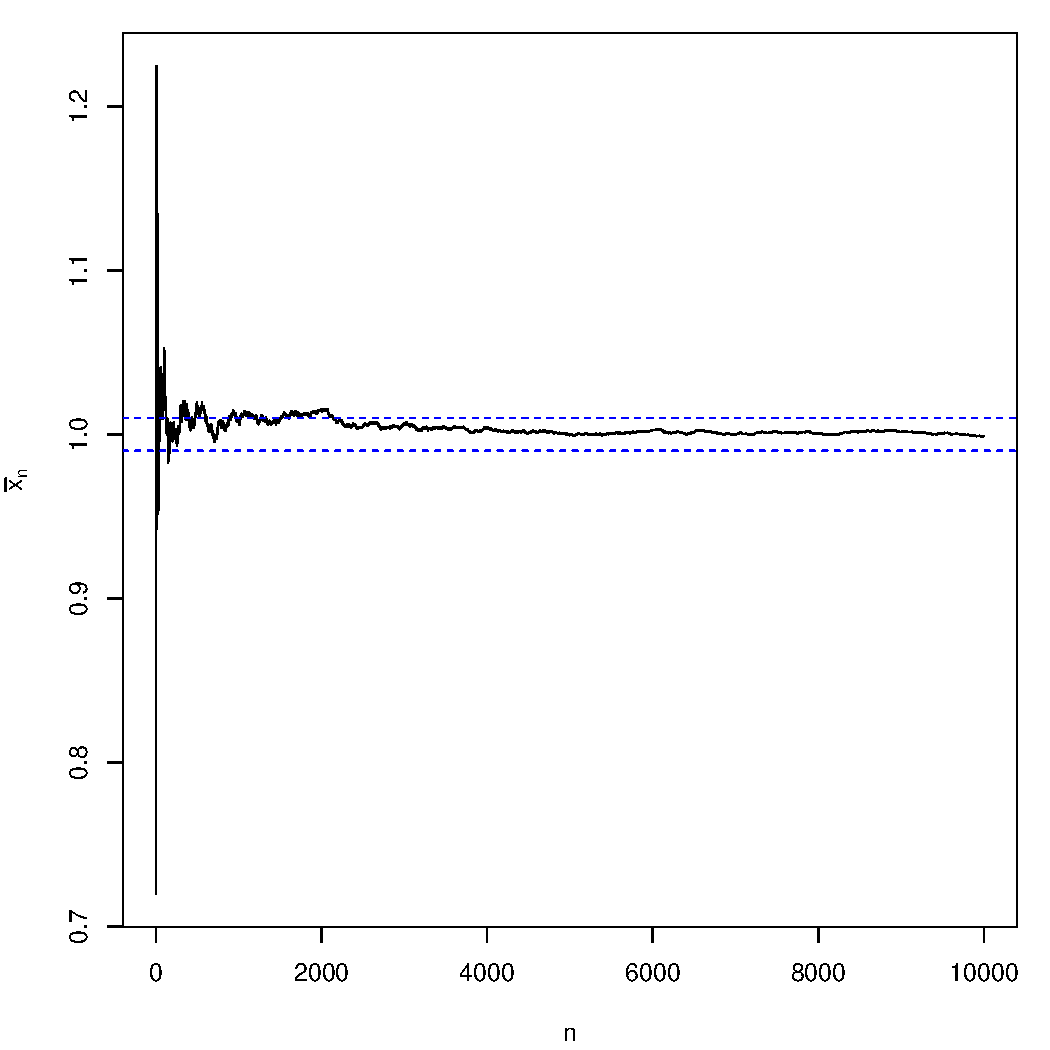
\includegraphics[width=10cm,height=10cm]{figure/CLT-normalplot-1} 

}


\end{knitrout}
\footnotesize
		\emph{Notes: This graphs shows the convergence of $\bar{X}$ as $n\to\infty$ for a normal distribution.}
	\end{minipage}
\end{figure}

From Figure \ref{fig:CLTnormal} we can see that $\overline{X}_n$ gets arbitrarily close to $\mu$ as $n$ increases indefinitely. In words, as the sample size $n$ increases, the sample mean converges to the theoretical mean. 
\end{example}

\begin{example}[Tossing a fair coin]
Now we simulate $n = 1000$ coin tosses. After each simulated toss, we plot the proportion $X_n$ of heads obtained so far against the number $n$ of tosses so far. The LLN says we should see a trace that gets very close to $1/2$ as $n$ increases.

In R, the code is:

\begin{knitrout}
\definecolor{shadecolor}{rgb}{0.969, 0.969, 0.969}\color{fgcolor}\begin{kframe}
\begin{alltt}
\hlcom{# Set up}
\hlkwd{set.seed}\hlstd{(}\hlnum{123}\hlstd{)}                            \hlcom{# set seed}
\hlstd{N} \hlkwb{<-} \hlnum{10000}                               \hlcom{# total number of tosses}
\hlstd{n} \hlkwb{<-} \hlnum{1}\hlopt{:}\hlstd{N}                                 \hlcom{# vector: n = 1, 2, ...., N; Toss number}

\hlcom{# Simulate and plot}
\hlstd{h} \hlkwb{<-} \hlkwd{rbinom}\hlstd{(}\hlkwc{n} \hlstd{= n,} \hlkwc{size} \hlstd{=} \hlnum{1}\hlstd{,} \hlkwc{prob} \hlstd{=} \hlnum{1}\hlopt{/}\hlnum{2}\hlstd{)} \hlcom{# vector: H = 0 or 1 each with p = 1./2}
\hlstd{x} \hlkwb{<-} \hlkwd{cumsum}\hlstd{(h)} \hlopt{/} \hlstd{n}                       \hlcom{# vector: proportion of heads}
\hlkwd{plot}\hlstd{(n, x,} \hlkwc{type} \hlstd{=} \hlstr{"l"}\hlstd{,} \hlkwc{ylim} \hlstd{=} \hlkwd{c}\hlstd{(}\hlnum{0}\hlstd{,} \hlnum{1}\hlstd{),} \hlkwc{ylab} \hlstd{=} \hlkwd{expression}\hlstd{(}\hlkwd{bar}\hlstd{(x)[n]))}
\hlkwd{abline}\hlstd{(}\hlkwc{h} \hlstd{=} \hlnum{0.52}\hlstd{,} \hlkwc{col} \hlstd{=} \hlstr{"blue"}\hlstd{,} \hlkwc{lty} \hlstd{=} \hlnum{2}\hlstd{)}
\hlkwd{abline}\hlstd{(}\hlkwc{h} \hlstd{=} \hlnum{0.48}\hlstd{,} \hlkwc{col} \hlstd{=} \hlstr{"blue"}\hlstd{,} \hlkwc{lty} \hlstd{=} \hlnum{2}\hlstd{)}
\end{alltt}
\end{kframe}
\end{knitrout}

\begin{figure}[H]
  \caption{Convergence of mean from binomial distribution}
    \label{fig:CLTbinomial}
     \centering
    \begin{minipage}{.9\linewidth}
\begin{knitrout}
\definecolor{shadecolor}{rgb}{0.969, 0.969, 0.969}\color{fgcolor}

{\centering 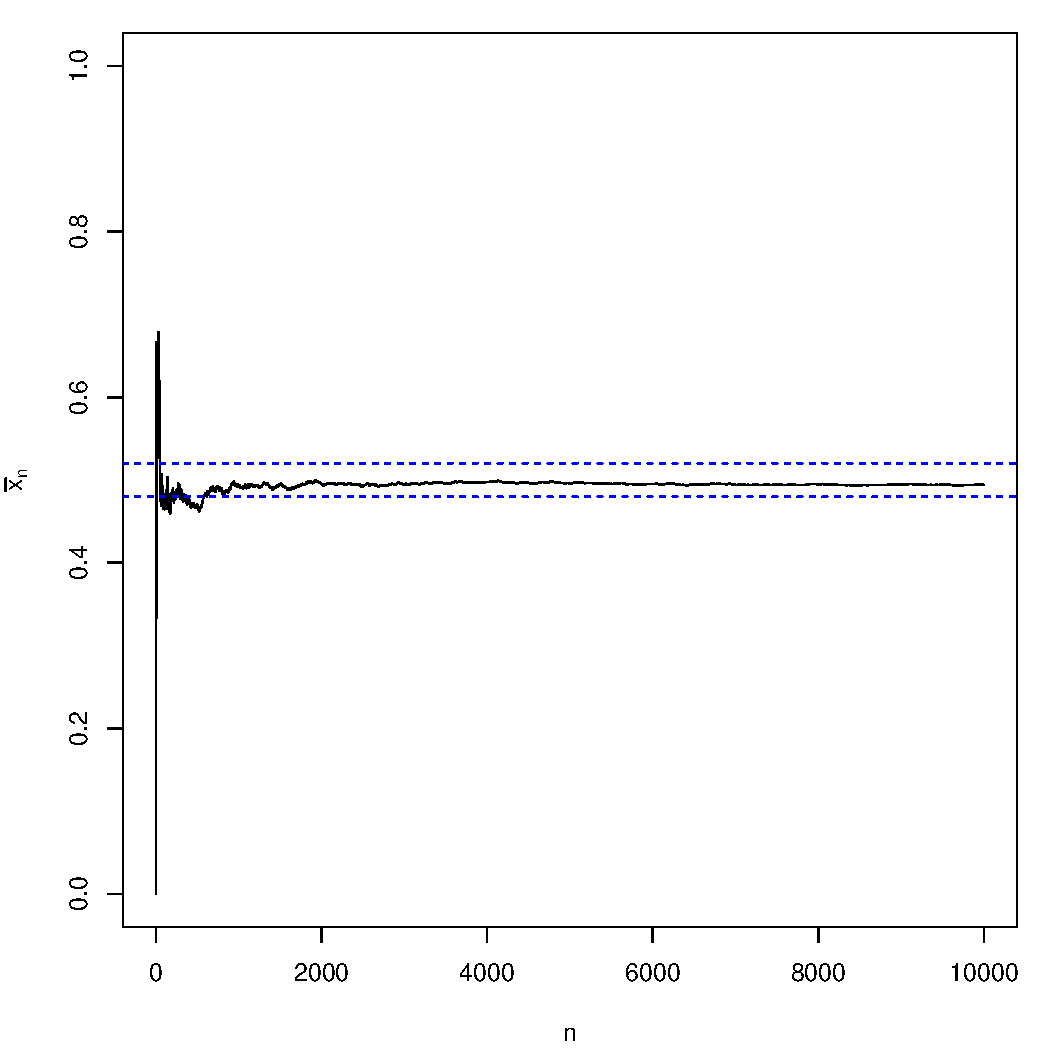
\includegraphics[width=10cm,height=10cm]{figure/CLT-binomialPlot-1} 

}


\end{knitrout}
\footnotesize
		\emph{Notes:} This graphs shows the convergence of $\bar{X}$ as $n\to\infty$ for a binomial distribution.
	\end{minipage}
\end{figure}

Note that the $n$th element of the vector \texttt{x} is the mean of the first $n$ elements of \texttt{h}. Figure \ref{fig:CLTbinomial} shows that the mean from a binomial distribution converges to the population mean $\mu = p = 1/2$, as $n\to \infty$. Note that the dashed lines at 0.48 and 0.52 illustrate the LLN with $\epsilon = 0.02$
\end{example}


Another important feature is that Khinchine's WLLN  is broader than Theorem \ref{teo:chebyshev} (Consistency of Unbiased Estimator), as \textbf{it does not require that the variance of the distribution be finite}. On the other hand, it is not broad enough, because most of the situations we encounter where we will need a result such as this will not involve i.i.d. random sampling. A broader LLN Theorem is the following:

\begin{theorem}[Chebychev's Weak Law of Large Numbers]\label{theorem:ChebychevWLLN}
  If $X_i, i = 1,...,n$ is a sample of observations such that $\E(X_i) = \mu_i <\infty$ and $\var(X_i)=\sigma^2_i < \infty$ such that
  
\begin{equation*}
  \frac{\bar{\sigma}^2_n}{n} = \frac{\sum_{i = 1}^n\sigma_i^2}{n^2}\to 0\quad \mbox{as $n\to\infty$},
\end{equation*}
%
then

\begin{equation*}
  \overline{X}_n - \bar{\mu}_n \pto 0.
\end{equation*}
\end{theorem}

The Chebychev's theorem does not state that $\overline{X}_n$ converges to $\bar{\mu}_n$, or even that it converges to a constant at all. The theorem states that as $n$ increases without bound, these two quantities will be arbitrarily close to each other. In other words, the difference between them converges to a constant, zero. The more important difference between the Khinchine and Chebyshev theorems is that the second allows for heterogeneity in the distributions of the random variables that enter the mean. This will be very useful in cases where the independence assumption may hold but the identical distribution assumption does not (such as random sampling with cross-sectional data). For example, the $X_i$'s may have different means and/or variances for each $i$. If we retain the independent assumption but relax the identical distribution assumption, then we can still get convergence of the sample mean.

It is important to stress that the behavior of the variance of $\overline{X}_n$ is the key element in this \textbf{LLN}. Independence implies that all covariances among the $X_i$ are zero, so that the variance of $\overline{X}_n$ simplifies to the sum of the variances of the $X_i$ divided by $n^2$. Then the key mechanism is that the variance of $\overline{X}_n$ converges to zero:

\begin{equation*}
 \lim_{n\to\infty}\var\left[ \overline{X}_n\right]=\lim_{n\to\infty}\frac{1}{n^2}\sum_{n=1}^n\var\left(X_i\right)=\lim_{n\to\infty}\frac{\sum_{i = 1}^n\sigma^2_i}{n}=0 
\end{equation*}

To illustrate Chebychev's WLLN we have created artificial data sets from independent normal distributions with different mean and standard deviations. Figure \ref{fig:chebychev} displays the sequence $\bar{X}_n - \bar{\mu}_n$ in black line and $\bar{\sigma}^2 / n^2$ as $n\to \infty$ in a red line. It can be observed that both sequences change with sample size, but as the number of observations increases both settle down to zero.  However, note that the sequence $\bar{X}_n - \bar{\mu}_n$ converges in probability, whereas $\bar{\sigma}^2 / n^2\to 0$ in a deterministic way. 


\begin{figure}[H]
  \caption{Chebychev's Convergence}
    \label{fig:chebychev}
         \centering
    \begin{minipage}{.9\linewidth}
\begin{knitrout}
\definecolor{shadecolor}{rgb}{0.969, 0.969, 0.969}\color{fgcolor}

{\centering 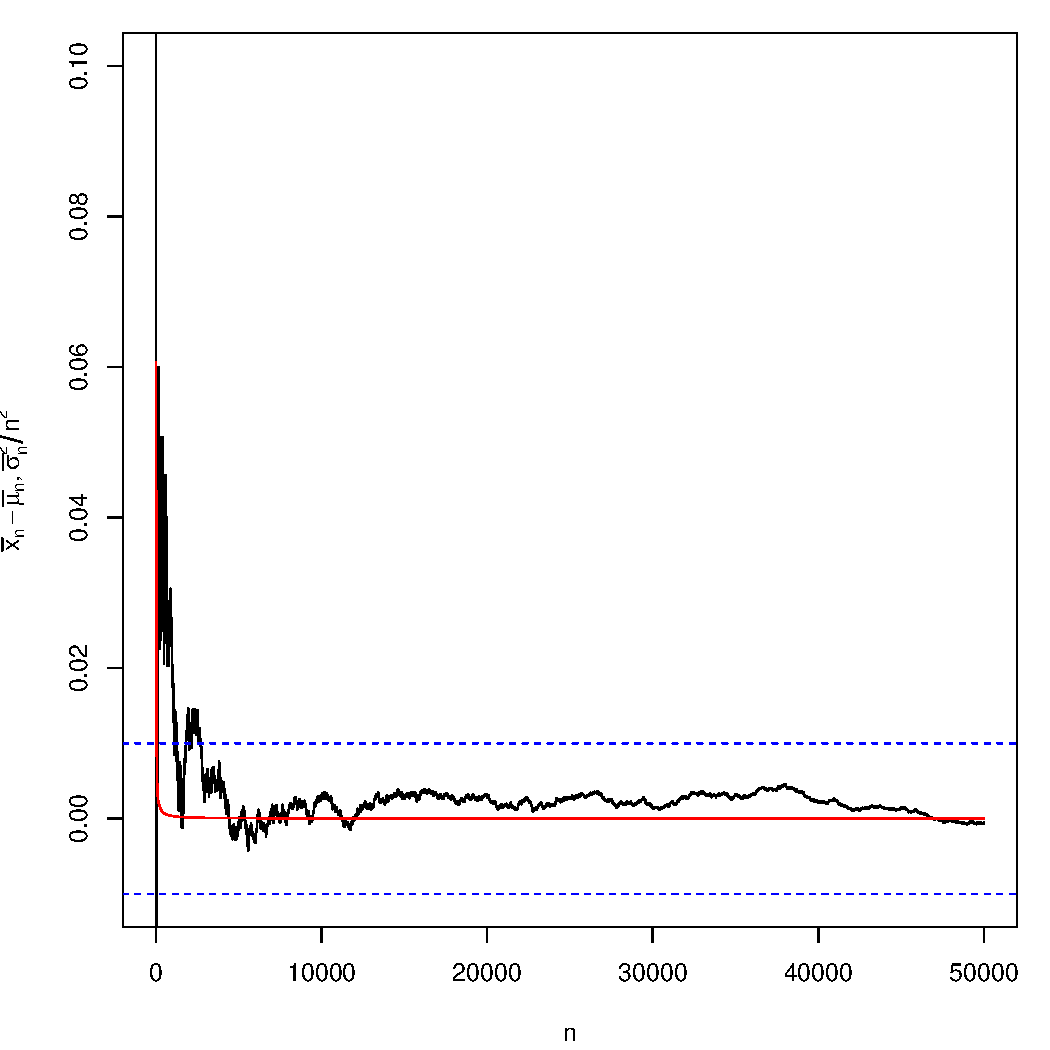
\includegraphics[width=10cm,height=10cm]{figure/cheby-convergence-1} 

}


\end{knitrout}
\footnotesize
		\emph{Notes: This graphs shows the convergence of $\bar{X}_n - \bar{\mu}_n$ and $\bar{\sigma}^2 / n^2$ as $n\to\infty$.}
	\end{minipage}
\end{figure}

\begin{remark}
  When the iid assumption is relaxed, stronger restrictions need to be place on the variances of each of the random variables. If some assumption are weakened then other assumptions must be strengthened. 
\end{remark}

To apply those LLN for several variables we have to know that summands of iid different random variables are also iid.

\begin{proposition}
	Let $\vg:\SR^K\to \SR^l$ be a continuous function. (i) Let $\mX_i$ and $\mX_t$ be identically distributed. Then $\vg(\mX_i)$ and $\vg(\mX_t)$ are identically distributed. (ii) Let $\mX_i$ and $\mX_t$ be independent. Then $\vg(\mX_i)$ and $\vg(\mX_t)$ are independent.
\end{proposition}

Therefore, using this proposition we can state the following proposition:

\begin{proposition}\label{proposition:iid_transf}
	If $\left\{(\mZ'_i,\mX_i,\vepsi_i)\right\}$ is an i.i.d random sequence, then $\left\{\mX_i\mX_i'\right\}$, $\left\{\mX_i\vepsi\right\}$, $\left\{\mZ_i\mX_i'\right\}$, $\left\{\mZ_i\vepsi_i\right\}$, and $\left\{\mZ_i\mZ_i'\right\}$ are also i.i.d sequences. 
\end{proposition}

This result is useful in situations in which we have observations from a random sample, as in a simple cross section. The result does not apply to stratified cross sections since there the observations are not identically distributed across strata, and generally will not apply to time-series data since there the observations $(\mX_i, \vepsi_i)$ generally are not independent. For these situations, we need laws of large numbers that do not  impose the i.i.d assumption.

What about expectations? The Jensen and Cauchy-Schwarz inequality will help us to work with Expectations of random variables. 

\begin{theorem}[Jensen's Inequality]\label{theorem:Jansen-Inequality}
If $g(X_n)$ is a concave function of $X_n$ then

\begin{equation*}
  g\left[\E(X_n)\right] \geq \E\left[g(X_n)\right]
\end{equation*}
\end{theorem}

\begin{theorem}[Cauchy-Schwarz Inequality]\label{theorem:Cauchy-Inequality}
For two random variables
\begin{equation*}
  \E\left[\left|X_nY_n\right|\right]\leq \left\lbrace \E\left[X_n^2\right]\right\rbrace^{1/2} \left\lbrace \E\left[Y_n^2\right]\right\rbrace^{1/2} 
\end{equation*}
\end{theorem}


%We can use this theorem in order to prove that the OLS variance estimator is consistent. Consider the i.i.d random variables $\epsilon_1^2, \epsilon_2^2, ..., \epsilon_N^2$, which have mean $\E\left[\epsilon_n^2\right] = \sigma^2$. From Khinchine's theorem it follows that:

%\begin{equation}
%\frac{1}{N}\sum_{i = 1}^N \epsilon_{i}^2 \pto \sigma^2
%\end{equation}

%which is the same as to say

%\begin{equation}
%\plim N^{-1}\vepsi'\vepsi = \sigma^2
%\end{equation} 

%To prove $\widehat{\sigma}^2 = \sigma^2$ consider the following estimator:

%\begin{eqnarray}
%\widehat{\sigma}^2 &=& \frac{\widehat{\vepsi}'\widehat{\vepsi}}{N - K}\nonumber \\
% & = & \frac{1}{N - K}\vepsi'\left(\mI - \mX\left(\mX'\mX\right)^{-1}\mX'\right)\vepsi \nonumber\\
% & = & \frac{N}{N - K}\left[\frac{\vepsi'\vepsi}{N} - \frac{\vepsi'\mX}{N}\left(\frac{\mX'\mX}{N}\right)^{-1}\frac{\mX'\vepsi}{N}\right]
%\end{eqnarray}

%Then, using Slutksy's theorem and the fact that $\plim \left[N/\left(N - K\right)\right] = 1$,

%\begin{eqnarray}
%\plim \widehat{\sigma}^2 & = & \plim \frac{\vepsi'\vepsi}{N} - \plim \frac{\vepsi'\mX}{N}\plim \left(\frac{\mX'\mX}{N}\right)^{-1}\plim \frac{\mX'\vepsi}{N} \\
%& = & \sigma^2 - 0 \cdot Q^{-1} \cdot 0 \\
%& = & \sigma^2
%\end{eqnarray}

%Before, we need the following theorems:

%\begin{theorem}[Chebychev's LLN]\label{theorem:Chebychev}
%Let $\left\lbrace X_n \right\rbrace$ be a sequence of i.i.d. random variables such that $\E\left[ X_n\right]$ and $\var\left[ X_n\right] $ exists $(n=1,2,3,...)$. Denote:

%\begin{equation*}
%E_N\left[X\right]\equiv \frac{1}{N}\sum_{n=1}^NX_n 
%\end{equation*}
%then $\E_N\left[X \right]\pto \E\left[ X\right]$ as $N\to\infty$
%\end{theorem}

%The behavior of the variance of $E_N\left[X \right]$ is the key element in this \textbf{LLN}. Independence implies that all covariances among the $X_n$ are zero, so that the variance of $\E_N\left[ X\right]$ simplifies to the sum of the variances of the $X_n$ divided by $N^2$. Then the key mechanism is that the variance of $\E_N\left[ X\right]$ converges to zero because the variance of the $X_n$ $(n-1,...,N)$ are all equal:

%\begin{equation*}
% \lim_{N\to\infty}\var\left[ \E_N\left[ X\right]\right]=\lim_{N\to\infty}\frac{1}{N^2}\sum_{n=1}^N\var[X]=\lim_{N\to\infty}\frac{\var[X]}{N}=0 
%\end{equation*}

%As a result, $\E_N[X]$ converges in distribution to the constant equal to its mean.


%==============================================
\section{Convergence in Distribution}
%==============================================


\begin{definition}[Convergence in Distribution]\label{definition:convergece_in_distribution}
	If the cdfs $F_{X_n}$ of the sequence of random variables $\left\lbrace X_n \right\rbrace $ converge to the cdf $F_{X}$ as $n\to \infty$ at all points $z$ where $F_{X}(z)$ is continuous, then $\left\lbrace X_n\right\rbrace $ converges in distribution to $X$. This will be denoted
	
	\begin{equation*}
	X_n\dto X
	\end{equation*}
%	
or 
	\begin{equation*}
	\lim_{n\to \infty}|F_{X_n}-F_{X}| = 0
	\end{equation*}
\end{definition}

This theorem states that the distribution of $X_n$ gets closer and closer to that of the random variable $X$, so that the distribution of $X$, the cdf $F_{X}$, can be used as an \textbf{approximation} to the distribution of $F_{X_n}$.  We can also say that $X$ es the \textbf{limiting distribution} of $X_n$.

%This statement is about the probability distribution associated with $X_n$; it does not imply that $X_n$ converges at all.

Convergence in distribution can be extended to random vectors and matrices although not in the element by element manner that we extended the earlier convergence forms. The reason is that convergence in distribution is a property of the CDF of the random variable, not the variable itself. Thus, $\vx_n\dto \vx$ if $\lim_{n\to \infty}|F_{\vx_n}-F_{\vx}| = 0$ and likewise for a random matrix. 


\begin{remark}
  One important case in which the limiting cdf $F$ is discontinuous is when $X$ is generate, meaning that it is identically equal to a constant $c$, so that $\Pr(X = c) = 1$. 
\end{remark}

\begin{remark}
In most applications, $X$ is either a normal or chi-square distributed random variable. 
\end{remark}


As an example, it is well know that 

\begin{equation*}
t_{n-1}\dto N(0, 1)
\end{equation*}

as $n\to \infty$.

\begin{theorem}[Convergence in probability implies convergence in distribution]\label{teo:pto_implies_dto}
  If the sequence of random variables $\left\lbrace X_n \right\rbrace$ convergences in probability to a random variable $X$, the sequence also converges in distribution to $X$. In other words:
  
  \begin{equation*}
    X_n\pto X\implies X_n\dto X
  \end{equation*}
\end{theorem}

Convergence in distribution is a weaker form of convergence than convergence in probability, in the sense that $\pto \implies \dto$. Intuitively, when $X_n$ converges to $X$ in probability as $n\to \infty$, the random variable $X_n$ will be arbitrarily close to random variable $X$ for $n$ sufficiently large. Therefore, the probability law of $X_n$ will be arbitrarily close to the probability law of $X$ for $n$ sufficiently large. That is, $X_n$ will converge in distribution to $X$ as $n\to \infty$.

However, $\dto$ does not imply $\pto$. When $\vx = \vtheta$ is a vector of constants the converse does hold. That is, it is also true that

\begin{equation*}
  \vx_n\dto \vtheta \implies \vx_n\pto \vtheta
\end{equation*}

In this case the limiting distribution of $\vx_n$ is degenerate since it collapses to the single point $\vtheta$.

\begin{example}[Defining Limiting Distribution Through Convergence in Probability]
Let $\left\lbrace Y_n\right\rbrace$ be defined by $Y_n = \left(2 + n^{-1}\right)X + 3$, where $X\sim \rN(1, 2)$. Using properties of $\plim$ operator if follows that

\begin{equation*}
  \plim \left(Y_n\right) = \plim \left[\left(2 + n^{-1}\right)X\right] + \plim(3) = 2X + 2 \sim \rN(5, 8). 
\end{equation*}
Then, Theorem \ref{teo:pto_implies_dto} implies that $Y_n\dto \rN(5, 8)$.
\end{example}

Another important result is that the moments of the asymptotic distribution of a random variable are not necessarily equal to the limits of the moments of the random variable's finite sample distribution. That is, in terms of the first two moments, $\vx_n\dto \vx$ does not necessarily imply that $\lim \E(\vx_n) = \E(\vx)$ and $\lim \E(\vx_n\vx_n') = \E(\vx\vx')$. For example, in simultaneous equation estimation, we frequently encounter estimator that do not possess finite moments of any order, but that, nevertheless, possess asymptotic distributions with well-defined moments.

\begin{example}
Consider a random sample $(y_1, y_2,...,y_n)$ from a normal distribution with mean $\mu \neq 0$ and variance $\sigma^2$. As an estimator for $\mu^{-1}$, the inverse of the sample mean $\bar{y}_n^{-1}$ is a natural choice. To establish its statistical properties we note that, from Khinchine's theorem, $\plim \bar{y}_n = \mu$, and then, from the continuous mapping theorem, $\plim \bar{y}_n^{-1} = \mu^{-1}$. Also because $\sqrt{n}(\bar{y}_n - \mu)\sim \rN(0, \sigma^2)$ for all $n$, it follows that

\begin{equation*}
  \sqrt{n}(\bar{y}_n - \mu)\dto \rN(0, \sigma^2)
\end{equation*}

Then, 

\begin{equation*}
  \sqrt{n}\left(\bar{y}_n^{-1} - \mu^{-1}\right)\dto \rN(0, \sigma^2\mu^{-4})
\end{equation*}

Thus the mean of the asymptotic distribution of $\bar{y}_n^{-1}$ is $\mu^{-1}$, but $\lim \E\left(\bar{y}_n^{-1}\right)\neq \mu^{-1}$ because it can be shown that $\E\left(\bar{y}_n^{-1}\right)$ does not exists. Note that this example also demonstrate that an estimator can be consistent, that is $\plim \bar{y}_n^{-1} = \mu^{-1}$, without its bias and variance going to zero as $n\to\infty$ ($\E\left(\bar{y}_n^{-1}\right)$ and $\var\left(\bar{y}_n^{-1}\right)$ do not exist.)
\end{example}

Some useful results that combine both probability and limiting distribution are as follows.

\begin{theorem}[Rules for limiting distribution]\label{teo:rules_dto}

Consider the following rules
\begin{enumerate}
  \item If $X_n\dto X$ and $Y_n\pto c$, then
      \begin{equation}\label{eq:rule_dtop}
         X_nY_n \dto cX
      \end{equation}
%
      which means that the limiting distribution of $X_nY_n$ is $cX$. Also, 
        \begin{equation}\label{eq:rule_dtop_2}
            X_n + Y_n \dto X + c
        \end{equation}
        
        \begin{equation}\label{eq:rule_dtop_3}
            X_n / Y_n \dto X / c, \quad \mbox{if $c\neq 0$}
        \end{equation}
        
    \item If $X_n\dto X$ and $g(X_n)$ is a continuous function, then
          \begin{equation}\label{eq:rule_dtop_4}
            g(X_n)\dto g(X)
          \end{equation}
    \item $\vx_n \dto \vx$, $\mA_n\pto \mA \implies \mA_n\vx_n \dto \mA\vx$, provided that $\mA_n$ and $\vx_n$ are conformable. In particular, if $\vx \sim \rN(\vzeros, \mSigma)$, then $\mA_n\vx_n\dto \rN(\vzeros, \mA\mSigma\mA')$.
    \item $\vx_n \dto \vx$, $\mA_n\pto \mA \implies \vx_n'\mA_n^{-1}\vx_n\dto \vx'\mA^{-1}\vx$, provided that $\mA_n$ and $\vx_n$ are conformable and $\mA$ is nonsingular.
\end{enumerate}
\end{theorem}

\begin{example}[Plims of Matrix Functions to Vector Random Variables]
Let $\left\lbrace \mX_n\right\rbrace$ and $\left\lbrace \mY_n\right\rbrace$ be such that $\plim\left(\mX_n\right) = \begin{pmatrix} 3 & 2 \\ 2 & 4 \end{pmatrix}$ and $\underset{(2\times 1)}{\mY_n}\dto\underset{(2\times 1)}{\mY}\sim \rN(\vzeros, \mI)$. Then, 

\begin{equation*}
  \mX_n\mY_n\dto \left[\plim\left(\mX_n\right)\right]\mY\sim \rN\left(\vzeros, \begin{pmatrix} 13 & 14 \\ 14 & 20\end{pmatrix}\right)
\end{equation*}

and

\begin{equation*}
  \mX_n^{-1}\mY_n\dto \left[\plim\left(\mX_n\right)\right]^{-1}\mY\sim \rN\left(\vzeros, \begin{pmatrix} .3125 & -.2188 \\ -.2188 & .2031\end{pmatrix}\right)
\end{equation*}
\end{example}

\begin{remark}
An useful example of Equation (\ref{eq:rule_dtop_4}) of Theorem \ref{teo:rules_dto} is the following. The exact distribution of $t_n^2$ is $F(1, n)$. But as $n\to \infty$, $t_n$ convergences to a standard normal variable. According to this result, the limiting distribution of $t_n^2$ will be that of the square of a standard normal, which is $\chi^2(1)$. Therefore, we conclude that:

\begin{equation*}
  F(1, n)\dto \chi^2(1)
\end{equation*}
\end{remark}


\begin{lemma}[Asymptotic Equivalence]\label{lemma:asymptotic_equiv}
  If $Y_n - X_n\pto 0$ and $X_n\dto X$ as $n\to \infty$, then $Y_n\dto X$
\end{lemma}

Intuitively, if two random variables $Y_n$ and $X_n$ are very close with probability approaching one as $n\to \infty$, they will follow the same large sample probability distribution. This lemma is very useful when one is interested in deriving the asymptotic distribution of $Y_n$. We can establish the asymptotic the asymptotic equivalence (in probability) between $Y_n$ and $X_n$ in the sense that $Y_n - X_n\pto 0$ as $n\to \infty$, then the asymptotic distributions of $Y_n$ and $X_n$ will be identical.\footnote{For example, this lemma is useful when deriving the distribution of spatial GLS is the same as the spatial FGSL. } 

\begin{theorem}[Cramer-Wold device]
If $\vx_n \dto \vx$, then $\vc'\vx_n \dto \vc'\vx$ for all conformable vectors $\vc$ with real valued elements.
\end{theorem}

%%%%%%%%%%%%%%%%%%%%%%%%%%%%%%%%%%%%
\section{Central Limit Theorems}
%%%%%%%%%%%%%%%%%%%%%%%%%%%%%%%%%%%%

Recall that we are interested in a way to describe the statistical properties of estimators when their exact distribution are unknown. However the previous tools do not allow us to find the limiting distribution. From Theorem \ref{teo:pto_implies_dto} (Convergence in probability implies convergence in distribution), we know that:

\begin{equation*}
  \widehat{\vtheta}_n\pto \vtheta \implies \widehat{\vtheta}\dto \vtheta.
\end{equation*}

That is, the limiting distribution of $\widehat{\vtheta}_n$ is a spike (the asymptotic distribution of $\widehat{\theta}_j$ collapses to a single point) and not very informative. The `trick' is to apply some normalization. For example, whereas $\widehat{\vtheta}_n\pto \vtheta$, we often find that

\begin{equation}
z_n = \sqrt{n}(\widehat{\vtheta}_n - \vtheta) \dto f(z),
\end{equation}
%
where $f(z)$ is a well-defined distribution with mean and positive variance. An estimator which has this properly is said to be \textbf{root-n consistent}.

\begin{mynote}
When learning econometrics is very difficult to understand how a estimator $\widehat{\theta}_n$ (random variable) converge to a single number but also converge to a (degenerate) distribution. We will see that under certain conditions $\widehat{\theta}_n$ converges in probability to $\theta_0$. This means that by choosing a large enough sample size $n$, the estimator will be as close as we want to the true parameter, with the probability of it being farther away as small as we want. Furthermore if we plot the distribution (or histogram) of $\widehat{\theta}_n$ for several $n$, it will eventually be just a spike centered on $\theta$ and not a normally distributed random variable. This is so because the variance of $\widehat{\theta}_n$ will go to zero eventually for a large enough $n$. Therefore, because $\var(\widehat{\theta}_n)\to 0$ the distribution shrink as $n\to \infty$. However, what does converge to a normally distributed random variable is $\sqrt{n}(\widehat{\theta}- \theta)$ because its variance does not grow with $n$. 
\end{mynote}

Central limit theorems, establish that, under some conditions, the arithmetic mean of a sufficiently large number of independent random variables, each with a finite expected value and finite variance, will be approximately normally distributed, regardless of the underlying distribution. 

The following Theorem gives the most classical (Central Limit Theorem) CLT. 


\begin{theorem}[Lindberg-Levy CLT (Univariate)]\label{theorem:LL_CLT_U}
Let $\left\lbrace X_n \right\rbrace$ be a sequence of i.i.d. random variables such that $\E(X_n) = \mu$ and the variance is strictly positive and finite, $0 < \sigma^2 < \infty$. Define $\overline{X}_n = n^{-1}\sum_{i = 1}^nX_i$. Then the distribution of

\begin{equation*}
  \begin{aligned}
      Z_n & = \frac{\overline{X}_n  - \E(\overline{X}_n)}{\sqrt{\var(\overline{X}_n)}} \\
          & = \frac{\overline{X}_n - \mu}{\sigma / \sqrt{n}} \\
      & = \frac{\sqrt{n}(\overline{X}_n - \mu)}{\sigma} \dto \rN(0, 1)
  \end{aligned}
\end{equation*}
%
as $n$ approaches infinity. This is the same as:
 
 
 \begin{equation*}
  \sqrt{n}(\overline{X}_n - \mu) = \frac{1}{\sqrt{n}}\sum_{i = 1}^n(X_i - \mu)\dto \rN(0, \sigma^2)
 \end{equation*}
\end{theorem}

This theorem tell us that if a large random sample is taken from any population distribution with finite variance, regardless of whether this population distribution is discrete or continuous, then the distribution of the standardized sample mean

\begin{equation*}
Z_n = \frac{\sqrt{n}(\overline{X}_n - \mu)}{\sigma}
\end{equation*}
%
will approximately follow a \rN(0, 1). Therefore, for each finite $n$, the distribution of $\overline{X}_n$ will be approximately a $\rN(\mu, \sigma^2/n)$.\\

It is important to stress that CLT does not say that a large population is approximately normally distributed. It says nothing about the distribution of the population; it is only a statement about the approximate distribution of a standardized sample mean $Z_n$. 

\begin{remark}
  Sometimes CLT is interpreted incorrectly as implying that the distribution of $\overline{X}_n$ approaches a normal distribution as $n\to \infty$. This is incorrect because $\var(\overline{X}_n)\to 0$ and $\overline{X}_n$ converges to a degenerate distribution $F(\cdot)$ such that $F(x) = 0$ if $x < \mu$ and $F(x) = 1$ if $x\geq \mu$.
\end{remark}

Multivariate versions of the CLTs can be obtained where each individual $\vx_i$ is a random vector in $\SR^K$, 


\begin{equation*}
\vx_i =\begin{pmatrix}
        x_{i1}\\
        x_{i2} \\
        \vdots\\
        x_{iK}
      \end{pmatrix}  
\end{equation*}
%
with mean vector:

\begin{equation*}
\vmu = \E(\vx_i) = \begin{pmatrix}
          \mu_1 \\
          \mu_2 \\
          \vdots \\
          \mu_K
       \end{pmatrix},
\end{equation*}
%
and covariance matrix $\mQ$. Then the sum of the random vectors will be componentwise, that is:

\begin{equation*}
\begin{pmatrix}
        x_{11}\\
        x_{12} \\
        \vdots\\
        x_{1K}
      \end{pmatrix} +
\begin{pmatrix}
        x_{21}\\
        x_{22} \\
        \vdots\\
        x_{2K}
      \end{pmatrix}+
\hdots +
\begin{pmatrix}
        x_{n1}\\
        x_{n2} \\
        \vdots\\
        x_{nK}
      \end{pmatrix} =
\begin{pmatrix}
\sum_{i = 1}^n x_{i1} \\
\sum_{i = 1}^n x_{i2} \\
\vdots \\
\sum_{i = 1}^n x_{iK}
\end{pmatrix}=
\sum_{i = 1}^n\vx_i.
\end{equation*}

The multivariate version of Theorem \ref{theorem:LL_CLT_U} is the following:


\begin{theorem}[Multivariate Lindberg-Levy CLT]\label{theorem:LL_CLT_M}
Let $\left\lbrace \vx_n \right\rbrace$ be a sequence of i.i.d. random variables from a multivariate distribution. If $\E(\vx_n) = \vmu$ and finite and positive covariance matrix $\mQ$. Then the distribution of

\begin{equation*}
  \begin{aligned}
      Z_n & = \sqrt{n}(\overline{\vx}_n - \vmu) \dto \rN(\vzeros, \mQ), 
  \end{aligned}
\end{equation*}
%
as $n$ approaches infinity, where $\overline{\vx}_n = (1 / n)\sum_{i = 1}^n\vx_i$.
\end{theorem}

The Linderbeg-Levy CLT is one of the several forms of this extremely powerful result. An important extension allow us to relax the assumption of equal variances. The Linderberg-Feller CLT allows for this extension:

\begin{theorem}[Univariate Lindberg-Feller CLT]\label{theorem:LF_CLT_U}
Let $\left\lbrace X_n\right\rbrace, i = 1, 2,...,n$ be a sequence of i.i.d. random variables. If $\E(X_i) = \mu_i$ and the variance is strictly positive and finite, $0 < \sigma^2_i < \infty$. Define 

\begin{equation*}
  \bar{\mu}_n = \frac{1}{n}(\mu_1 + \mu_2 + ... +\mu_n), \quad \mbox{and} \quad \bar{\sigma}^2_n =\frac{1}{n}(\sigma^2_1 + \sigma^2_2 + ... +\sigma^2_n)
\end{equation*}

If no single term dominates this average variance, which we could state as

\begin{equation*}
\lim_{n\to \infty} \frac{\max (\sigma_i)}{n \bar{\sigma}_n} = 0,
\end{equation*}
%
and if the average variance converges to a finite constant,

\begin{equation*}
\lim_{n\to \infty} \bar{\sigma}^2_n = \bar{\sigma}^2
\end{equation*}
%
then

\begin{equation*}
  \begin{aligned}
      Z_n &  = \frac{\sqrt{n}(\overline{X}_n - \bar{\mu})}{\bar{\sigma}} \dto \rN(0, 1)
  \end{aligned}
\end{equation*}
%
 as $n$ approaches infinity.
\end{theorem}

In practical terms, the theorem states that sums of random variables, regardless of their form, will tend to be normally distributed. 


\begin{theorem}[Multivariate Lindberg-Feller CLT]\label{theorem:LF_CLT_M}
Suppose that $\vx_1, \vx_2,...,\vx_n$ are a sample of random vectors such that $\E(\vx_i) = \vmu_i$, $\var(\vx_i) = \mQ_i$, and all mixed third moments of the multivariate distribution are finite. Let

\begin{equation*}
  \bar{\vmu}_n = \frac{1}{n}\sum_{i = 1}^n\vmu_i,
\end{equation*}

\begin{equation*}
  \overline{\mQ}_n = \frac{1}{n}\sum_{i = 1}^n\mQ_i.
\end{equation*}

We assume that

\begin{equation*}
  \lim_{n \to \infty}\overline{\mQ}_n  = \mQ,
\end{equation*}
%
where $\mQ$ is a finite, positive definite matrix, and that for every $i$,

\begin{equation*}
  \lim_{n \to \infty}(n\overline{\mQ}_n)^{-1}\mQ_i = \lim_{n \to \infty}\left(\sum_{i = 1}^n \mQ_i\right)^{-1} \mQ_i = \vzeros
\end{equation*}

We allow the means of the random vectors to differ, although in the cases that will analyze, they will generally be identical. The second assumption states that individual components of the sum must be finite and diminish in significance. There is also an implicit assumption that the sum of matrices is nonsingular. Because the limiting matrix is nonsingular, the assumption must hold for large enough $n$, which is all that concerns us here. With these in place, the result is

\begin{equation*}
  \sqrt{n}(\bar{\vx}_n - \bar{\vmu}_n)\dto \rN(\vzeros, \mQ)
\end{equation*}
\end{theorem}

\begin{theorem}[Liapounov Central Limit Theorem]
Suppose that $\left\lbrace X_n\right\rbrace, i = 1, 2,...,n$ is a sequence of independent random variables with finite mean $\mu_i$ and finite positive variances $\sigma^2_i$ such that $\E\left[\left|X_i - \mu_i\right|^{2 + \delta}\right]$ if finite for some $\delta > 0$. If $\bar{\sigma}_n$ is positive and finite for all $n$ sufficiently large, then

\begin{equation*}
  \frac{\sqrt{n}(\overline{X}_n - \bar{\mu}_n)}{\bar{\sigma}_n}\dto\rN(0, 1)
\end{equation*}
\end{theorem}

This version of the central limit theorem requires only that moments slightly larger than two be finite and it is generally used when the variables are fixed. 

We end this section by defining the concept of \textbf{asymptotic variance}.


\begin{definition}[Asymptotic Variance]\label{def:asymptotic_variance}
Let $\left\lbrace\vx_n\right\rbrace$ be a sequence of random vectors. If there exists a sequence of matrices $\left\lbrace \mV_n\right\rbrace$ such that $\mV_n$ is nonsingular for all $n$ sufficiently large and $\mV^
{-1/2}\vx_n \adistr \rN(\vzeros, \mI)$, then $\mV_n$ is called the asymptotic covariance matrix of $\vx_n$, denoted $\avar(\vx_n)$.
\end{definition}


%-----------------------------------
\section{Orden in Probability}
%-----------------------------------


Similarly to the nonsthocastic sequences, we can make similar statement about $o$ and $O$ when we have random variables. The following theorem state the definition of unboudedness and convergence for random variables: 

\begin{definition}[Order in Probability]\label{definition:order_prob}
Consider the following two definition:

\begin{enumerate}
		\item \textbf{Stochastically Bounded (Big O)}: The sequence of random variables  $\left\{X_n\right\}$ is at most of order in probability $n^\lambda$, and we write
		
		\begin{equation}
			X_n = O_p(n^\lambda)
		\end{equation}
		
		if, for every $\epsilon > 0$, there exists a real number $n_0$ such that:
		
		\begin{equation}
			\Pr\left[n^{-\lambda} \left|X_n \right| \geq n_0 \right]\leq \epsilon
		\end{equation}
		
		for all $n$. 
		
		\item \textbf{Stochastic Convergence}: Also, we say that $\left\{X_n\right\}$ is of smaller order in probability than $n^\lambda$ and we write
		
		\begin{equation}
		X_n = o_p\left(n^\lambda\right)
		\end{equation}
		
		if 
		
		\begin{equation}
			\plim n^{-\lambda}X_n = 0
		\end{equation}
		
		When $\lambda = 0$, $X_n$ converges to zero, and we also write $X_n=o_p(1)$.
		
	\end{enumerate}
\end{definition}

Intuitively, for $X_n = O_p(n^\lambda)$ with $\lambda > 0$, the order $n^\lambda$ is the fastest growth rate at which $X_n$ goes to infinity with probability approaching 1. When $\lambda < 0$, the order $n^\lambda$ is the fastest convergence rate at which $X_n$ vanishes to 0 with probability approaching 1. Thus, $X_n= O_p(1) = O_p(n^0)$ implies that for $n$ sufficiently large, $\left|X_n\right|$ takes value larger than a very large constant has a tiny probability. In other words, $\left|X_n\right|$ is bounded by a constant with a very high probability for all $n$ sufficiently large. 

\begin{definition}[Stochastically Negligible]
	If $X_n\pto 0$, then $X_{n} = o_p(1)$. If $X_n = n^\lambda o_p(1)$, then $X_n = o_p(n^{-\lambda})$	
\end{definition}

To give some intuition about these definitions, consider $\vx_n \dto \vx$ and $\vy_n\pto \vzeros$. Then:

\begin{equation*}
  \vx_n + \vy_n \dto \vx\quad \mbox{by \ref{eq:rule_dtop} in Theorem \ref{teo:rules_dto}}
\end{equation*}

That is, if  $\vz_n = \vx_n + \vy_n$ and $\vy_n\pto \vzeros$, implying that $\vz_n - \vx_n \pto \vzeros$, then the asymptotic distribution of $\vz_n$ is the same as that of $\vx_n$. Note that this is the same as Lemma \ref{lemma:asymptotic_equiv} (asymptotic equivalence). So we can write:

\begin{equation*}
  \vz_n \adistr \vx_n\quad \mbox{or}\quad \vz_n = \vx_n + o_p(1)
\end{equation*}
%
where $o_p(1)$ is some variable ($\vy_n$ in this case) that is sthochastically negligible, that is, it converges to zero in probability. 

This is more intuitive if we think in the consistency of OLS estimator. Given the OLS consistency, it is the same to write:

\begin{equation*}
\widehat{\vbeta}_n \pto \vbeta_0\quad \mbox{as $n\to\infty$}
\end{equation*}
%
as

\begin{equation*}
\widehat{\vbeta}_n = \vbeta_0  + o_p(1) \quad \mbox{as $n\to\infty$}
\end{equation*}

In other words, a consistent estimator is equal to the true estimator plus something that converges to 0 in probability. 

%------------------------------------------------------------------
\begin{lemma}[Convergence in distribution implies boundedness]
  Let $X_n$ be a random variable with CDF $F_n(\cdot)$, and let $X$ be a random variable with continuous CDF $F(\cdot)$. If $X_n\dto X$ as $n\to \infty$, then $X_n = O_p(1)$
\end{lemma}
%------------------------------------------------------------------

Intuitively, if the probability distribution of $X_n$ converges to a well-defined continuous probability distribution as $n\to \infty$, then $X_n$ is bounded in probability. This result is very useful for establishing that a sequence of random variables is bounded in probability. Often it is easier to verify that a sequence of random variables converges in distribution. 

When do we use the $O_p$?  If a random vector converges in distribution $\vx_n \dto \vx$ (for example $\vx\sim \rN(\vzeros, \mV)$) then $\vx_n = O_p(1)$. 

\begin{example}
  If $X_n\sim N(0,1)$ for all $n\geq 1$. Then $X_n = O_p(1)$ because for any given $\delta > 0$, there exists a finite constant $M = \Phi^{-1}(1 - \delta/2)<\infty$, where $\Phi$ is the $\rN(0, 1)$ CDF, such that
  
  \begin{equation*}
    \Pr(\left|X_n\right| > M) = 2\left[1 - \Phi(M)\right] = \delta < 2\delta
  \end{equation*}
  %
  for all $n \geq 1$
\end{example}

$O_p(1)$ is weaker than $o_p(1)$ in the sense that $X_n = o_p(1)$ implies $X_n = O_p(1)$ but not the reverse.

There are many simple rules for manipulating $o_p(1)$ and $O_p(1)$ sequences which can be deduced from the continuous mapping theorem or Slutsky's Theorem. For example:

\begin{eqnarray*}
 o_p(1) + o_p(1) & = & o_p(1) \\
 o_p(1) + O_p(1) & = & O_p(1) \\
 O_p(1) + O_p(1) & = & O_p(1) \\
 o_p(1) o_p(1)   & = & o_p(1) \\
 o_p(1) O_p(1)   & = & o_p(1) \\
 O_p(1) O_p(1)   & = & O_p(1)
\end{eqnarray*}

One of the most common uses of this concept of stochastic order is ``root-$n$'' $(\sqrt{n})$ consistency:

\begin{definition}[$\sqrt{N}$-Consistent]
		if $\sqrt{n}\left(\vtheta_n - \vtheta_0\right)= O_p(1)$, then $\vtheta_n$ is $\sqrt{n}$ consistent for $\vtheta_0$
\end{definition}

\begin{example}[OLS and $O_p$ and $o_p$]
Recall that:

\begin{equation*}
  \widehat{\vbeta}_n = \vbeta_0 + (\mX'\mX)^{-1}\mX'\vepsi.
\end{equation*}

Under appropriate assumption, we know that:

\begin{equation*}
  \frac{1}{n}\mX'\mX\pto \E(\mX'\mX),
\end{equation*}
%
which is finite and positive definite. The fact that the elements of $n^{-1}\mX'\mX$ converge to finite limits in probability implies that $N^{-1}\mX'\mX$ is \textbf{bounded} in the sense that the sequences of the elements within $n^{-1}\mX'\mX$ are bounded, and under these circumstances we say that $\mX'\mX$ is at most of order $n$, that is, $\mX'\mX = O_p(n)$, or we can say:

\begin{equation*}
n^{-1}\mX'\mX = O_p(1).
\end{equation*}

We also assume that $n^{-1/2} \mX'\vepsi$ has probability limit which a normally distributed random variable with expectation zero and finite variance. So, we can write:

\begin{equation*}
\mX'\vepsi = O_p(n^{1/2}).
\end{equation*}

Thus:


\begin{equation*}
  \begin{aligned}
\widehat{\vbeta}_n - \vbeta_0 & =  (\mX'\mX)^{-1}\mX'\vepsi  \\
\widehat{\vbeta}_n - \vbeta_0 & =  (n^{-1}\mX'\mX)^{-1}n^{-1}\mX'\vepsi  \\
\widehat{\vbeta}_n - \vbeta_0 & = O_p(1) \cdot o_p(1) \\
\widehat{\vbeta}_n - \vbeta_0 & = o_p(1)
\end{aligned}
\end{equation*}

Also:

\begin{equation*}
  \begin{aligned}
\widehat{\vbeta}_n - \vbeta_0 & =  (\mX'\mX)^{-1}\mX'\vepsi  \\
\widehat{\vbeta}_n - \vbeta_0 & =  \left[O_p(n)\right]^{-1}O_p(n^{1/2}) \\
\widehat{\vbeta}_n - \vbeta_0 & =  O_p(n^{-1})O_p(n^{1/2}) \quad \because \left[O_p(n)\right]^{-1}= O_p(n^{-1})\\
\widehat{\vbeta}_n - \vbeta_0 & =  O_p(n^{-1/2})\\
\end{aligned}
\end{equation*}
%

So, we might then say that $\widehat{\vbeta}_n - \vbeta_0$ is converging to zero at the rate $1/\sqrt{n}$; and the rate tell us what multiplier of the variable $\widehat{\vbeta}_n - \vbeta_0$ stabilizes it so that it convergences to a well-defined random variables rather than to 0 or $\infty$. 

Note also that: 

\begin{equation*}
  \begin{aligned}
    \sqrt{n}(\widehat{\vbeta}_n - \vbeta_0) & =  n^{1/2}O_p(n^{-1})O_p(n^{1/2})\\
    & = n^{1/2} O_p(n^{-1/2}) \\
    & = O_p(1) \quad \because X_n = O_p(1/\sqrt{n}) \implies X_n / (1/\sqrt{n})= \sqrt{n} X_n = O_p(1) 
  \end{aligned}
\end{equation*}
\end{example}

\begin{example}[Rate of convergence for sample mean]
Consider and iid random sample $X_i$ with mean $\mu = 0$ and variance $\sigma^2 = 0,25$. Then, by the CLT the sample mean $\bar{X}$ we know that $\sqrt{n}(\bar{X}-\mu) /\sigma \dto \rN(0 , 1)$. That is, $\sqrt{n}(\bar{X}-\mu)/\sigma = O_p(1)$. This implies that $\bar{X} - \mu= O_p(\sqrt{n})$. Figure \ref{fig:Op_example} shows how $\bar{X}$ converges towards $\mu$ to the speed of $1\sqrt{n}$.
\end{example}


\begin{figure}[H]
  \caption{Convergence of the sample mean and speed of convergence}
    \label{fig:Op_example}
        \centering
    \begin{minipage}{.9\linewidth}
\begin{knitrout}
\definecolor{shadecolor}{rgb}{0.969, 0.969, 0.969}\color{fgcolor}

{\centering 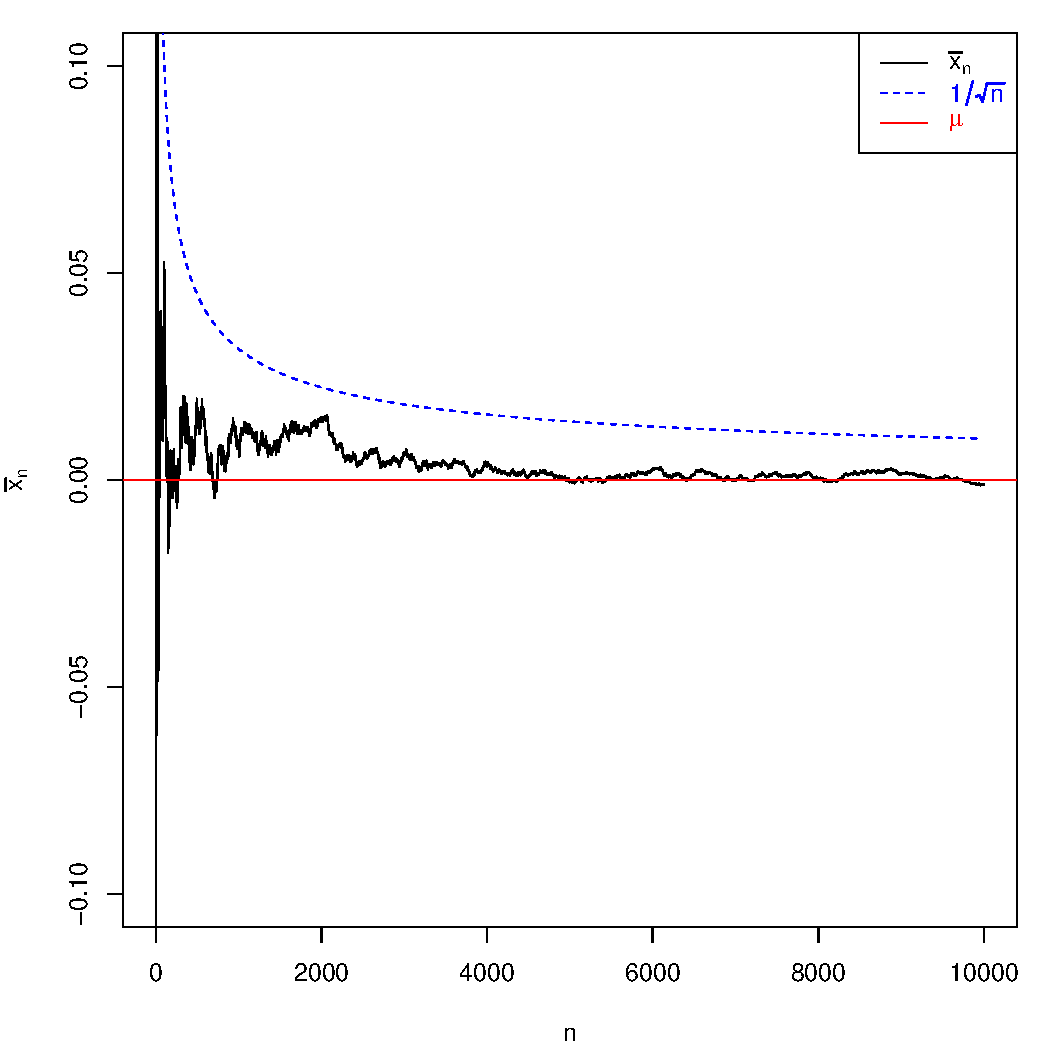
\includegraphics[width=10cm,height=10cm]{figure/CLT-normalplot-bigO-1} 

}


\end{knitrout}
\footnotesize
		\emph{Notes: This graphs shows the convergence of $\bar{X}$ to $\mu$ as $n\to\infty$ for a normal distribution as fast as $1/\sqrt{n}$.}
	\end{minipage}
\end{figure}

%----------------------------------
\section{Triangular Arrays}\label{sec:triangular-array}
%----------------------------------

An important question is the context of asymptotic theory is the following: \emph{What is the meaning of $n\to \infty$ in a spatial context?} Will increase the geographical area or will increase the number of spatial unit in a given geographical area? 

For spatial data, two distinct asymptotic frameworks have been studied: \textbf{increasing domain} and \textbf{infill asymptotic}. Increasing domain consists of a sampling structure where new observations (spatial units) are added at the edges (boundary points), similar to the underlying asymptotic in time series analysis. That is, increasing domain asymptotic refers to more and more observations being sampled over an increasing domain. The problem here is what the boundary is. When referring to increasing domain asymptotic, it is assumed that the spatial locations of the observations do not become dense. Infill asymptotic are appropriate when the spatial domain is bounded, and new observations (points) are added in between existing ones, generating denser surface. In most applications of spatial econometric, the implied structure is that of an increasing domain. 

The increasing domain framework requires the knowledge of \textbf{triangular arrays}.  The following definition give us a simply definition of Triangular Arrays. 

\begin{definition}[Triangular Array of Random Variables]\label{def:triangular-array} 
The ordered collection of random variables 

\begin{equation*}
\left\lbrace X_{11}, X_{21}, X_{22}, X_{31}, X_{32}, X_{33}, ... , X_{nn}, ...\right\rbrace,
\end{equation*}
%
or

\begin{equation*}
\begin{pmatrix}
X_{11} &        &        &        &        &        & \\
X_{21} & X_{22} &        &        &        &        & \\
X_{31} & X_{32} & X_{33} &        &        &        & \\
\vdots & \vdots & \vdots & \ddots &        &        & \\
X_{n1} & X_{n2} & X_{n3} & X_{n4} & \hdots & X_{nn} & \\
\vdots & \vdots & \vdots & \vdots & \vdots & \vdots & \ddots
\end{pmatrix}
\end{equation*}

is called a triangular array of random variables, and will be denoted by $\left\lbrace X_{nn}\right\rbrace$.
\end{definition}

Central limit theorems that are applied to triangular arrays of random variables are concerned with limiting distributions of appropriately defined function of the row average $S_n = n^{-1}\sum_{i = 1}^nX_{ni}$. For example, for $n = 3$ (third row) we have $S_3 = (1/3)(X_{31} + X_{32} + X_{33})$.  Note that the traditional CLTs deal with functions of average of the type $n^{-1}\sum_{i = 1}^n X_i$, the $X_i$'s being elements of the sequence $\left\lbrace X_n\right\rbrace$. However, the triangular array $\left\lbrace X_{nn}\right\rbrace$ is more general than a sequence $\left\lbrace X_n\right\rbrace$ in the sense that the random variables in a row of the array need not be the same as random variables in other rows. Thus, the triangular nature of a random variable leads to certain statistical problems, especially with respect to the relevant CLT that should be applied. In other words, we will need a CLT applicable to triangular array. Both the LLN and CLT require slightly stronger conditions than the LLN and CLT for i.i.d sequence of random variables. 

What are the conditions on the random variables so that a properly $S_n$ converges to a normal distribution as $n\to \infty$. In a nutshell, assume: 

\begin{itemize}
  \item Independence: assume all random variables in the array are independent.
  \item Centering: assume $\E(X_{j,i}) = 0$ for all $j, i$.
  \item Variances converge: assume $\sum_{i = 1}^n\E(X_{n, i}^2)\to \sigma^2> 0$ as $n\to\infty$
  \item No single variance is too large.
\end{itemize}

Then $S_n \dto N(0, \sigma^2)$ as $n\to\infty$.

Probably you're asking yourself, why triangular arrays are important in the spatial context? Note that if we adopt the increasing domain approach, it is clear that as $n$ increases,  $\mW$ itself changes as observations are added. To see this,  let $\vtheta_0 = (\vbeta_0^\top, \rho_0, \sigma_0^2)^\top$ be the true parameter vector. We further assume that variables and estimates depend on the sample size $n$. This will allow us to study their behavior as $n\to \infty$.  Therefore, denote $\mA_n(\rho) = \mI_n - \rho \mW_n$ for any value of $\rho$. The ``equilibrium'' vector is

\begin{equation}\label{eq:equilibrium_slm}
\vy_n = \mA_n^{-1}(\mX_n\vbeta_0 + \vepsi_n)
\end{equation}
%
where $\mA_n = \mA_n(\rho_0)$ is nonsingular. Let $\vepsi_n(\vdelta) = \vy_n - \mX_n\vbeta - \rho \mW_n\vy_n$, where $\vdelta = (\vbeta^\top, \rho)^\top$. Thus, $\vepsi_n = \vepsi_n(\vdelta_0)$. Since the matrices $(\mI_n - \rho\mW)^{-1}$ generally depend upon the sample size $n$, the vectors $\vy$ and $\vepsi$ will also depend upon $n$, and they will form a \textbf{triangular arrays}. This is due to the fact that for the ``boundary'' elements the sample weights matrix changes as new spatial units --- or new data points --- are added. That is, new spatial units change the structure for the existing spatial units \citep[see for example][]{kelejian1999generalized, kelejian2001asymptotic, anselinSpatialEcon}. For example, the outcome for the first spatial unit, $y_{1,n}$, will be different if we consider a total  $n = 10$ or $n = 15$ observations because of the changing nature of $\mW$ as $n$ changes and given the DGP in Equation (\ref{eq:equilibrium_slm}). This implies that these elements and the vector $\vy$ should be indexed by $n$:

\begin{equation*}
  \vy_n = (y_{11}, y_{21}, y_{22},..., y_{nn})
\end{equation*}

For example, for $n = 1, 2, 3$, then (by row):

\begin{equation*}
\begin{aligned}
  n = 1 & \implies y_{11} \;         \\
  n = 2 & \implies y_{12} \; y_{22}  \\
  n = 3 & \implies y_{13} \; y_{23} \; y_{33} \\
  \vdots & \\
  n = n & \implies y_{13} \; y_{23} \; y_{33} \hdots y_{3n}
\end{aligned}
\end{equation*}
%
where $y_{11} \neq y_{12} \neq y_{13}$ and $y_{22}\neq y_{23}$. Note that the dependent variable in the same row are mutually independent (spatial units are independent) and have the same distribution. But the distribution of  the random variable $y$ (and $\epsilon$) in different rows are allowed to be different. 

The triangular array structure of $y$ is partly a consequence of allowing a triangular array structure for the disturbances in the model. But there is a more fundamental reason for it, and for treating the $\mX$ observations as a triangular array also. In allowing for the elements of $\mX_n$ to depend on $n$ we allow explicitly for some of the regressors to be spatial lags.

We can identify each of the indices $i = 1,...,n$ with a location in space. In regularly-observed time series settings, these indices correspond to equidistant points on the real line, and it is evident what we usually mean by letting $n$ increase. However there is ambiguity when these points are in space. For example, consider $n$ points on a 2 dimensional regularly-spaced lattice, where both the number ($n_1$) of rows and the number $(n_2)$ of columns increases with $n=n_1\cdot n_2$. If we choose to list these points in lexicographic order (say first left to right, then second row, etc) then as $n$ increases there would have to be some re-labeling, as the triangular array permits. Another consequence of this listing is that dependence between locations $i$ and $j$ is not always naturally expressed as a function of the difference $i-j$. For example, this is so if the dependence is isotropic. 


%----------------------------------
\section{Bounded Matrices}
%----------------------------------

\begin{definition}[Bounded Matrices]\label{def:Bounded_Matrices}
Let $\left\lbrace \mA_n \right\rbrace$ be a sequence of $n$-dimensional square matrices, where $\mA_n = \left[a_{n,ij}\right]$,
  \begin{enumerate}
    \item The column sums of $\left\lbrace \mA_n \right\rbrace$ are uniformly bounded (in absolute value) if there exists a finite constant $c$ that does not depend on $n$ such that 
    
    \begin{equation*}
      \left\|\mA_n\right\|_{\infty} = \max_{1 \leq j\leq n}\sum_{i = 1}^n\left|a_{n, ij}\right| \leq c
    \end{equation*}
     \item The row sums of $\left\lbrace \mA_n \right\rbrace$ are uniformly bounded (in absolute value) if there exists a finite constant $c$ that does not depend on $n$ such that 
    
    \begin{equation*}
      \left\|\mA_n\right\|_1 = \max_{1 \leq i\leq n}\sum_{j = 1}^n\left|a_{n, ij}\right| \leq c
    \end{equation*}
  \end{enumerate}
\end{definition}

Then $\left\lbrace \mA_n \right\rbrace$ is said to be \textbf{uniformly bounded} in row sums if $\left\lbrace\left\|\mA_n\right\|_1\right\rbrace$ is a bounded sequence. Similarly, $\left\lbrace \mA_n \right\rbrace$ is said to be \textbf{uniformly bounded} in column sums if $\left\lbrace\left\|\mA_n\right\|_{\infty}\right\rbrace$ is a bounded sequence. 

The following lemmas will be very useful:

\begin{lemma}\label{lemma:bounded_lemma}
If $\left\lbrace \mA_n \right\rbrace$ an $\left\lbrace \mB_n \right\rbrace$ are uniformly bounded in row sums (column sums), then $\left\lbrace \mA_n \mB_n\right\rbrace$ is also uniformly bounded in row sums (column sums).
\end{lemma}

\begin{lemma}\label{lemma:bounde_ON}
If $\left\lbrace \mA_n \right\rbrace$ is absolutely summable, and $\mZ_n$ has bounded elements, then the elements of $\mZ_n^\top \mA_n\mZ_n = O(n)$
\end{lemma}


%---------------------------------
\section{Quadratic forms}
%---------------------------------

\begin{definition}[Quadratic form]\label{def:quad-form}
For a $n\times n$ symmetric matrix $\mA_n=\left[a_{ij}\right]$ the quadratic function of $n$ variables $\vepsi$ defined by:

\begin{equation}
\vepsi^\top \mA_n \vepsi = \sum_{i = 1}^n\sum_{j = 1}^na_{ij}\epsilon_i\epsilon_j
\end{equation}
%
is called the quadratic form with matrix $\mA_n$.  If $\mA_n$ is not symmetric, we can replace $\mA_n$ by $\left(\mA_n + \mA_n^\top\right)/2$.
\end{definition}

%--------------------------------------------------------------
\begin{lemma}[First and Second Moments]\label{lemma:second-mom-lee}
Let $\mA_n=\left[a_{ij}\right]$ be an $n$-dimensional square matrix. Then, it can be shown that:

\begin{equation*}
\E\left[\vepsi^\top_n\mA_n\vepsi_n\right]=\tr\left(\mA_n\mSigma\right)+\vmu^\top\mA_n\vmu
\end{equation*}
%
where $\vmu$ and $\mSigma$ are the expected value and variance-covariance matrix of $\vepsi_n$, respectively. This result only depends on the existence of $\vmu$ and $\mSigma$; it does not require normality of $\vepsi$. 

Assume that $\mu = \vzeros$ and $\mSigma = \sigma_0^2\mI$, then

\begin{enumerate}
  \item $\E(\vepsi_n^\top\mA_n\vepsi_n) = \sigma^2_0\tr(\mA_n)$,
  \item $\E(\vepsi_n^\top\mA_n\vepsi_n)^2 = (\mu_4 - 3\sigma^4_0)\sum_{i = 1}^na_{ii}^2+\sigma^4_0\left[\tr^2(\mA_n) + \tr(\mA_n\mA_n^\top)+\tr(\mA^2_n)\right]$, and
  \item $\var(\vepsi_n^\top\mA_n\vepsi_n) = (\mu_4 - 3\sigma^4_0)\sum_{i = 1}^na_{ii}^2+\sigma^4_0\left[\tr(\mA_n\mA_n^\top)+\tr(\mA^2_n)\right]$.
\end{enumerate}

For the moment assume that $\mA$ is symmetric and $\vepsi$ is normally distributed, then:

\begin{equation*}
\var\left(\vepsi^\top\mA\vepsi\right)= 2\tr\left(\mA\mSigma\mA\mSigma\right) + 4\vmu^\top\mA\mSigma\mA\vmu,
\end{equation*}
%
and the covariance:

\begin{equation*}
\cov\left(\vepsi^\top\mA_1\vepsi, \vepsi^\top\mA_2\vepsi\right)= 2\tr\left(\mA_1\mSigma\mA_2\mSigma\right) + 4\vmu^\top\mA_1\mSigma\mA_2\vmu
\end{equation*}

If $\mA$ is not symmetric, then:

\begin{equation}\label{eq:var-quadratic-form}
\cov\left(\vepsi^\top\mA_1\vepsi, \vepsi^\top\mA_2\vepsi\right)= 2\tr\left[\frac{1}{2}\left(\mA_1 + \mA_1^\top\right)\mSigma\frac{1}{2}\left(\mA_2 + \mA_2^\top\right)\mSigma\right] + 4\vmu^\top\frac{1}{2}\left(\mA_1 + \mA_1^\top\right)\mSigma\frac{1}{2}\left(\mA_2 + \mA_2^\top\right)\vmu
\end{equation}

In particular, if $\vepsi$'s are normally distributed with mean 0 and variance $\sigma_0^2$, then 

\begin{itemize}
  \item $\E(\vepsi_n^\top\mA_n\vepsi_n)^2 = \sigma^4_0\left[\tr^2(\mA_n) + \tr(\mA_n\mA_n^\top)+\tr(\mA^2_n)\right]$, and
  \item $\var(\vepsi_n^\top\mA_n\vepsi_n) = \sigma^4_0\left[\tr(\mA_n\mA_n^\top)+\tr(\mA^2_n)\right]$
\end{itemize}
\end{lemma}
%--------------------------------------------------------------

\begin{proof}
We can write:
\begin{equation*}
\begin{aligned}
\vepsi'\mA\vepsi & = \left(\vepsi - \mu\right)'\mA\vepsi + \vmu'\mA\vepsi
\end{aligned}
\end{equation*}
\end{proof}

\begin{lemma}\label{lemma:O-lemma-lee}
Suppose that  $\left\lbrace \mA_n\right\rbrace$ is uniformly bounded in either row and column sums, and the elements $a_{n, ij}$ of $\mA_n$ are $O(1/h_n)$ uniformly in all $i$ and $j$. Then:

\begin{itemize}
  \item $\E(\vepsi_n^\top\mA_n\vepsi_n) = O(n/h_n)$,
  \item $\var(\vepsi_n^\top\mA_n\vepsi_n)=O(n/h_n)$, and
  \item $\vepsi_n^\top\mA_n\vepsi_n = O_p(n/h_n)$.
\end{itemize}

Furthermore:

\begin{itemize}
\item $\lim_{n\to\infty}\frac{h_n}{n} = 0$, and,
\item $\frac{h_n}{n}\vepsi_n^\top\mA_n\vepsi_n - \frac{h_n}{n}\E(\vepsi_n^\top\mA_n\vepsi_n) = o_p(1)$
\end{itemize}
\end{lemma}


\begin{theorem}[Consistency of quadratic forms in spatial models]\label{teo:quadratic-forms-ley}
Let $\mS$ be an $n\times n$ nonstochastic matrix whose row and columns sums are uniformly bounded in absolute value. Let $\vv^{\top}=(v_1, ..., v_n)$ where $v_i$ are iid $(0, \sigma^2)$ and $\E(v_i^4)<\infty$. Then

\begin{equation*}
  \frac{\vv^\top \mS \vv}{n}\pto \E\left(\vv^\top \mS \vv\right) = \sigma^2\frac{\tr(\mS)}{n}
\end{equation*}

If the limit of $\tr(\mS)/n$ exits, then:

\begin{equation*}
\lim_{n\to\infty}\frac{\tr(\mS)}{n} = \mS^*
\end{equation*}
%
and

\begin{equation*}
  \frac{\vv^\top \mS \vv}{n}\pto \sigma^2\mS^*.
\end{equation*}
\end{theorem}




%---------------------------------
\section{CLT for Spatial Models}
%---------------------------------


The following theorem states the limiting distribution for triangular arrays with homokedastic errors in linear forms:

\begin{theorem}[CLT for triangular arrays with homokedastic errors, \citep{kelejian1998generalized}]\label{teo:CLT_tri_arr}
Let $\left\lbrace v_{i,n}, 1 \leq i \leq n, n\geq 1\right\rbrace $ be a triangular array of identically distributed random variables. Assume that the random variables $\left\lbrace v_{i,n}, 1 \leq i \leq n\right\rbrace$ are jointly independently distributed for each $n$ with $\E(v_{i,n})= 0$ and $\E(v_{i,n}^2) = \sigma^2 < \infty$. Let $\left\lbrace a_{ij,n}, 1 \leq i \leq n, n\geq 1\right\rbrace, j = 1,...,k$ be triangular arrays of real numbers that are bounded in absolute value. Further let

\begin{equation*}
  \vv_n = \begin{pmatrix}
            v_{1, n} \\
            \vdots \\
            v_{n,n}
          \end{pmatrix}, \quad
          \mA_n = \begin{pmatrix}
            a_{11,n} & \hdots & a_{1k, n} \\
            \vdots &         & \vdots \\
            a_{n1,n} & \hdots & a_{nk, n}
          \end{pmatrix}
\end{equation*}

Then:

\begin{equation*}
\frac{1}{\sqrt{n}}\mA_n^\top\vv_n = O_p(1)
\end{equation*}

Furthermore, assume that $\lim_{n\to\infty}n^{-1}\mA^\top_n\mA_n = \mQ_{AA}$ is finite and nonsingular matrix. Then

\begin{equation*}
\frac{1}{\sqrt{n}}\mA_n^\top\vv_n \dto \rN(\vzeros, \sigma^2 \mQ_{AA})
\end{equation*}
\end{theorem}


\begin{theorem}[CLT for Vectors of Linear Quadratic Forms with Heterokedastic Innovations]\label{teo:clt_quadratic}
		Assume the following:
		\begin{enumerate}
			\item For $r = 1,...,m$ let $\mA_{r,n}$ with elements $(a_{ijr})_{i,j = 1,...,n}$ be an $n\times n$ non-stochastic symmetric real matrix with $\sup_{1\leq j \leq n, n\geq 1}\sum_{i = 1}^n|a_{ijr}| < \infty$,
			\item and let $\va_r = (a_{ir},...,a_{nr})^\top$ be a $n \times 1$ non-stochastic real vector with $\sup_{n}\frac{\sum_{i=1}^n \left|a_{ir}\right|^{\delta_1}}{n}<\infty$ for some $\delta_1 > 2$.
			\item Let $\vepsi = (\epsilon_1,...,\epsilon_n)^\top$ be an $n \times 1$ random vector with the $\epsilon_i$ distributed totally independent with $\E\left[\epsilon_i\right] = 0, \E\left[\epsilon_i^2\right]$, and  $\sup_{1 \leq i \leq n, n \geq 1}\E\left|\epsilon_{i}\right|^{\delta_2}<\infty$ for some $\delta_2 >4$. 
		\end{enumerate}
		Consider the $m \times 1$ vector of linear quadratic forms $\vv_n = \left[Q_{1n},..., Q_{mn}\right]'$ with:
		
		\begin{equation}
			Q_{rn}= \vepsi'\mA_r\vepsi + \va_r'\vepsi = \sum_{i=1}^n\sum_{j=1}^na_{ijr}\epsilon_i\epsilon_j + \sum_{i=1}^na_{ir}\epsilon_i.
		\end{equation}
		
		Let $\mu_{\vv} = \mE\left[\vv_n\right] = \left[\mu_{Q_1},...,\mu_{Q_2}\right]^\top$ and $\mSigma_{\vv_n} =\left[\sigma_{Q_{rs}}\right]_{r,s =1,...,m}$ denote the mean and VC matrix of $\vv_n$, respectively, then:
		
		\begin{equation*}
			\begin{aligned}
			\mu_{Q_r} & = \sum_{i = 1}^na_{iir}\sigma_i^2 \\
			 \sigma_{Q_{rs}} & = 2\sum_{i=1}^n\sum_{j =1}^na_{ijr}a_{ijs}\sigma^2_i\sigma_j^2 + \sum_{i = 1}^na_{ir}a_{is}\sigma_i^2 \\
			 	            & + \sum_{i = 1}^na_{iir}a_{iis}\left[\mu_i^{(4)} - 3\mu_i^{4}\right] + \sum_{i =1}^n(a_{ir}a_{iis} + a_{is}a_{iir})\mu_i^{(3)}
			\end{aligned}
		\end{equation*}
		
		with $\mu_i^{(3)} = \mE(\epsilon_i^3)$ and $\mu_i^{(4)} = \mE(\epsilon_i^4)$. Furthermore, given that $n^{-1}\lambda_{min}(\mSigma_{\vv_n})\geq c$ for some $c > 0$, then
		
		\begin{equation*}
		\mSigma_{\vv_n} ^{-1/2}(\vv_n - \mu_{\vv_n})\dto \rN(\vzeros, \mI_m)
		\end{equation*}
		
		and thus:
		
		\begin{equation*}
			n^{-1/2}(\vv_n - \mu_{\vv_n}) \adistr \rN(\vzeros, n^{-1}\mSigma_{\vv_n})
		\end{equation*}
\end{theorem}	

\cite{kelejian2001asymptotic} introduced a CLT for a single quadratic form under the assumptions useful for spatial models. The generalization to vectors of linear quadratic forms is given in \cite{kelejian2010specification}.
